\chapter{Desenvolvimento}\label{cap:desenvolvimento}

Este capítulo tem como objetivo detalhar a concepção e a estruturação do projeto ``Preço Bão''. Nas seções a seguir, serão apresentados os elementos fundamentais para a compreensão do escopo do sistema, iniciando pela delimitação do minimundo, que descreve o domínio do problema, os fluxos operacionais e os principais requisitos que guiarão a modelagem do banco de dados e a arquitetura do software.

\section{Minimundo}

O projeto consiste em uma plataforma de serviço, acessível via aplicativo móvel e site, voltada para ajudar o consumidor final a pesquisar, comparar e monitorar os preços de medicamentos e produtos de farmácia.

A arquitetura prevê a alimentação por rotinas automatizadas de extração de dados (\textit{web scraping}\footnote{Técnica computacional automatizada em que um \textit{script} ou algoritmo navega por páginas da web com o objetivo de raspar, coletar e estruturar em um banco de dados as informações públicas que originalmente são exibidas de forma não estruturada em código HTML.}) que varre os sites de diversas farmácias da região. Durante esse processo, o sistema coleta, processa e armazena informações vitais, como a disponibilidade dos produtos, os laboratórios fabricantes e os valores cobrados, construindo um grande catálogo centralizado de remédios.

Através da interface do aplicativo, o usuário final pode pesquisar pelos medicamentos de uso contínuo ou produtos que precisa comprar. A interface implementada apresenta os produtos em cartões de exibição, listando as informações do laboratório e comparando os melhores preços encontrados no mercado. Como funcionalidade prevista (RF06), o aplicativo deverá receber coordenadas mediante permissão e calcular distâncias até os estabelecimentos. Esse fluxo não está integrado às rotas de pesquisa consultadas; coordenadas de farmácias no modelo não comprovam geolocalização do consumidor.

O código contém favoritos vinculados à conta e consulta de observações de preço por produto e farmácia. Esses registros auxiliam o acompanhamento de variações, sem garantir o melhor momento ou local de compra. Preços, disponibilidade e cobertura dependem das fontes e dos instantes de coleta.

\section{Especificação de Requisitos}

Nesta seção, os requisitos do sistema ``Preço Bão'' são detalhados e classificados. Os Requisitos Funcionais (RF) descrevem as ações e comportamentos que o sistema deve executar para atender às necessidades do usuário, enquanto os Requisitos Não Funcionais (RNF) especificam os critérios de qualidade, restrições tecnológicas e de desempenho que o sistema deve respeitar.

\begingroup\footnotesize\def\LTcaptype{quadro}
\begin{xltabular}{\textwidth}{|c|Y|}
\caption{Especificação dos Requisitos Funcionais}\label{qua:requisitos_funcionais}\\
        \hline
        \textbf{ID} & \textbf{Descrição do Requisito} \\
        \hline\endfirsthead
\multicolumn{2}{l}{Quadro \thequadro\ -- continuação}\\
        \hline
        \textbf{ID} & \textbf{Descrição do Requisito} \\
        \hline\endhead
\multicolumn{2}{r}{Continua na próxima página.}\\\endfoot
\multicolumn{2}{l}{Fonte: Elaborado pelos autores (2026).}\\\endlastfoot

        RF01 & \textbf{Extração Resiliente de Dados:} O sistema deve possuir uma rotina automatizada de \textit{web scraping} para coletar dados de farmácias. Em caso de falha na extração, o sistema deve registrar o erro em \textit{log} e continuar a varredura nas demais fontes. \\
        \hline
        RF02 & \textbf{Processamento e Catálogo:} O sistema deve armazenar as informações vitais extraídas e enriquecê-las contra a base da CMED/ANVISA. A disponibilidade em estoque deve ser exibida com um aviso claro de que é uma ``estimativa sujeita a confirmação no local''. \\
        \hline
        RF03 & \textbf{Gestão de Usuários:} O aplicativo deve permitir o cadastro de novos usuários, autenticação (\textit{login}) e recuperação de senha, criando um perfil individual. \\
        \hline
        RF04 & \textbf{Pesquisa e Neutralidade Algorítmica:} O consumidor deve poder pesquisar por medicamentos. O algoritmo de ordenação deve garantir a neutralidade, priorizando estritamente o menor preço ou a menor distância. \\
        \hline
        RF05 & \textbf{Exibição em Cartões:} O sistema deve exibir os resultados em cartões padronizados, listando informações do laboratório e comparando os melhores preços. \\
        \hline
        RF06 & \textbf{Cálculo de Distância Geográfica:} Mediante autorização prévia, o aplicativo deve receber as coordenadas geográficas do usuário e calcular a distância até os estabelecimentos, ordenando por proximidade. \\
        \hline
        RF07 & \textbf{Salvamento de Produtos:} O sistema deve permitir que um usuário autenticado favorite medicamentos de uso contínuo em sua conta. \\
        \hline
        RF08 & \textbf{Monitoramento de Preços:} O sistema deve gerar e exibir um gráfico ou histórico rastreando a flutuação de preços dos remédios salvos ao longo das últimas semanas. \\
        \hline
    \end{xltabular}
\endgroup

\vspace{0.5cm}

\begingroup\footnotesize\def\LTcaptype{quadro}
\begin{xltabular}{\textwidth}{|c|Y|}
\caption{Requisitos Não Funcionais: Arquitetura e Performance}\label{qua:rnf_arquitetura}\\
        \hline
        \textbf{ID} & \textbf{Descrição do Requisito} \\
        \hline\endfirsthead
\multicolumn{2}{l}{Quadro \thequadro\ -- continuação}\\
        \hline
        \textbf{ID} & \textbf{Descrição do Requisito} \\
        \hline\endhead
\multicolumn{2}{r}{Continua na próxima página.}\\\endfoot
\multicolumn{2}{l}{Fonte: Elaborado pelos autores (2026).}\\\endlastfoot

        RNF01 & \textbf{Performance da API:} O \textit{backend} (Python/FastAPI) deve ser assíncrono e responder a requisições de pesquisa em um tempo máximo de 500 milissegundos no percentil 95. \\
        \hline
        RNF02 & \textbf{Arquitetura do Frontend:} O aplicativo móvel deve ser desenvolvido com React Native e Expo utilizando TypeScript, com a meta de obter \textit{builds} funcionais para Android e iOS. \\
        \hline
        RNF03 & \textbf{Persistência e Retenção:} Os dados devem ser armazenados em um PostgreSQL. O sistema deve implementar uma política de limpeza (\textit{data purging}), excluindo históricos com mais de 12 meses. \\
        \hline
    \end{xltabular}
\endgroup

\vspace{0.5cm}

\begingroup\footnotesize\def\LTcaptype{quadro}
\begin{xltabular}{\textwidth}{|c|Y|}
\caption{Requisitos Não Funcionais: Segurança e Conformidade}\label{qua:rnf_seguranca}\\
        \hline
        \textbf{ID} & \textbf{Descrição do Requisito} \\
        \hline\endfirsthead
\multicolumn{2}{l}{Quadro \thequadro\ -- continuação}\\
        \hline
        \textbf{ID} & \textbf{Descrição do Requisito} \\
        \hline\endhead
\multicolumn{2}{r}{Continua na próxima página.}\\\endfoot
\multicolumn{2}{l}{Fonte: Elaborado pelos autores (2026).}\\\endlastfoot

        RNF04 & \textbf{Segurança e Criptografia:} Todas as senhas devem ser armazenadas utilizando \textit{hashing} fortes (ex: bcrypt). A comunicação deve ocorrer obrigatoriamente sob protocolo HTTPS/TLS. \\
        \hline
        RNF05 & \textbf{Privacidade (LGPD):} O sistema não deve armazenar o histórico contínuo de localização do usuário. As coordenadas devem ser processadas em memória e descartadas em seguida. \\
        \hline
    \end{xltabular}
\endgroup

\vspace{0.5cm}

\begingroup\footnotesize\def\LTcaptype{quadro}
\begin{xltabular}{\textwidth}{|c|Y|}
\caption{Requisitos Não Funcionais: Engenharia e Qualidade de Código}\label{qua:rnf_engenharia}\\
        \hline
        \textbf{ID} & \textbf{Descrição do Requisito} \\
        \hline\endfirsthead
\multicolumn{2}{l}{Quadro \thequadro\ -- continuação}\\
        \hline
        \textbf{ID} & \textbf{Descrição do Requisito} \\
        \hline\endhead
\multicolumn{2}{r}{Continua na próxima página.}\\\endfoot
\multicolumn{2}{l}{Fonte: Elaborado pelos autores (2026).}\\\endlastfoot

        RNF06 & \textbf{Estrutura e Validação:} O sistema deve utilizar ORM e Pydantic no \textit{backend} para validação. O TypeScript no \textit{frontend} deve usar modo estrito (\code{strict: true}). \\
        \hline
        RNF07 & \textbf{Organização em Monorepo:} O projeto deve adotar a estrutura de monorepo, isolando as dependências do \textit{frontend} e do \textit{backend}. \\
        \hline
        RNF08 & \textbf{Orquestração Local:} O ambiente de desenvolvimento deve ser provisionado via \file{docker-compose.yml}. \\
        \hline
        RNF09 & \textbf{Automação de Comandos:} O repositório deve conter um \file{Makefile} na raiz para abstrair comandos complexos (ex.: \code{make db-up}). \\
        \hline
        RNF10 & \textbf{CI/CD e Qualidade:} Fluxos do GitHub Actions devem bloquear \textit{Pull Requests} que falhem nos testes ou na análise estática (ESLint/Ruff). \\
        \hline
        RNF11 & \textbf{Padronização de Estilo:} O repositório deve impor formatação via \file{.editorconfig} e possuir um \file{.gitignore} configurado para excluir arquivos sensíveis do versionamento. \\
        \hline
    \end{xltabular}
\endgroup

\subsection{Situação dos requisitos na implementação}\label{sec:situacao}

Os Quadros \ref{qua:requisitos_funcionais} a \ref{qua:rnf_engenharia} expressam objetivos do projeto. A conferência estática dos fontes distingue presença de componentes de validação por execução. Os testes do plano permanecem pendentes.

\begin{itemize}
\item \textbf{RF01--RF02:} há coleta em \file{app/scrapers/}, persistência e enriquecimento local em \file{app/services/enriquecimento.py}. O ETL CMED é acionável por comandos; isso não prova agendamento periódico nem cobertura de todas as fontes. O aviso de estoque estimado exige conferência da interface e não decorre de um campo booleano.
\item \textbf{RF03:} as rotas em \file{app/api/routes/usuarios.py} integram cadastro, autenticação e perfil. Os callbacks de recuperação em \file{app/core/auth.py} apenas registram a solicitação; não há inclusão do roteador de recuperação nem entrega de token demonstrada no fluxo público.
\item \textbf{RF04--RF06:} há pesquisa e ordenação por preço, nome e relevância em \file{app/api/routes/catalogo.py}, além de cartões no frontend. A menor distância permanece prevista. Não se infere neutralidade completa da existência de uma ordenação: critérios e resultados precisam de teste.
\item \textbf{RF07--RF08:} favoritos possuem vínculos persistentes por usuário e verificação de autenticação. A consulta de histórico em \file{app/api/routes/historico.py} agrupa observações por farmácia e período; é pública e não exige que o produto esteja favoritado. A persistência é implementada em \file{app/services/preco_observacoes.py}; o gráfico é composto por \file{HistoryChart.tsx}.
\end{itemize}

Quanto aos requisitos não funcionais, FastAPI e rotinas assíncronas estão presentes, mas o acesso SQLAlchemy usa sessões síncronas; não se afirma atendimento integral ao RNF01 nem ao p95 de 500 ms sem medição. React Native, Expo e TypeScript constam dos fontes (RNF02); exportação não comprova fluxos funcionais Android e iOS. PostgreSQL está configurado, mas filtros temporais do histórico não constituem exclusão automática após 12 meses (RNF03).

A autenticação utiliza a infraestrutura FastAPI Users e armazenamento em \ident{hashed_password}. O Compose contém túnel para a API, mas não comprova HTTPS/TLS em todos os ambientes; o coletor Indiana contém cliente com verificação de certificado desativada (RNF04). A ausência de histórico contínuo de localização no modelo não comprova conformidade integral à LGPD nem o fluxo de descarte ainda não implementado (RNF05).

ORM, Pydantic, configuração TypeScript estrita, organização em monorepo, Compose e Makefile sustentam os componentes de RNF06--RNF09. O alvo real de provisionamento do banco é \code{make db-up}. Não foram localizados workflows em \file{.github/workflows/}; scripts locais de análise não comprovam bloqueio de PRs nem implantação contínua (RNF10). \file{.editorconfig} existe, mas está vazio e não impõe regras; \file{.gitignore} exclui arquivos sensíveis comuns (RNF11). Esses arquivos não garantem ausência de segredos em todo o histórico.

\section{Modelagem do Sistema}

A modelagem usa a UML para relacionar o comportamento esperado aos componentes. A abordagem de casos de uso é descrita por \citeonline{booch2005}; a organização de modelos de domínio e projetos de classes é discutida por \citeonline{larman2007}. Os diagramas a seguir representam o escopo planejado ou a estrutura técnica, conforme indicado em cada figura.

\subsection{Diagrama de Casos de Uso}\label{sec:casos_uso}

A Figura \ref{fig:diagrama_casos_de_uso} delimita a plataforma e relaciona o consumidor aos serviços de pesquisa, comparação, conta, favoritos e histórico. O operador aciona coleta e ingestão; sites de farmácias e arquivo CMED são fontes externas. O robô interno não é modelado como ator externo da própria plataforma.

\begin{figure}[htb]
\centering
\caption{Casos de uso do escopo previsto da plataforma}\label{fig:diagrama_casos_de_uso}
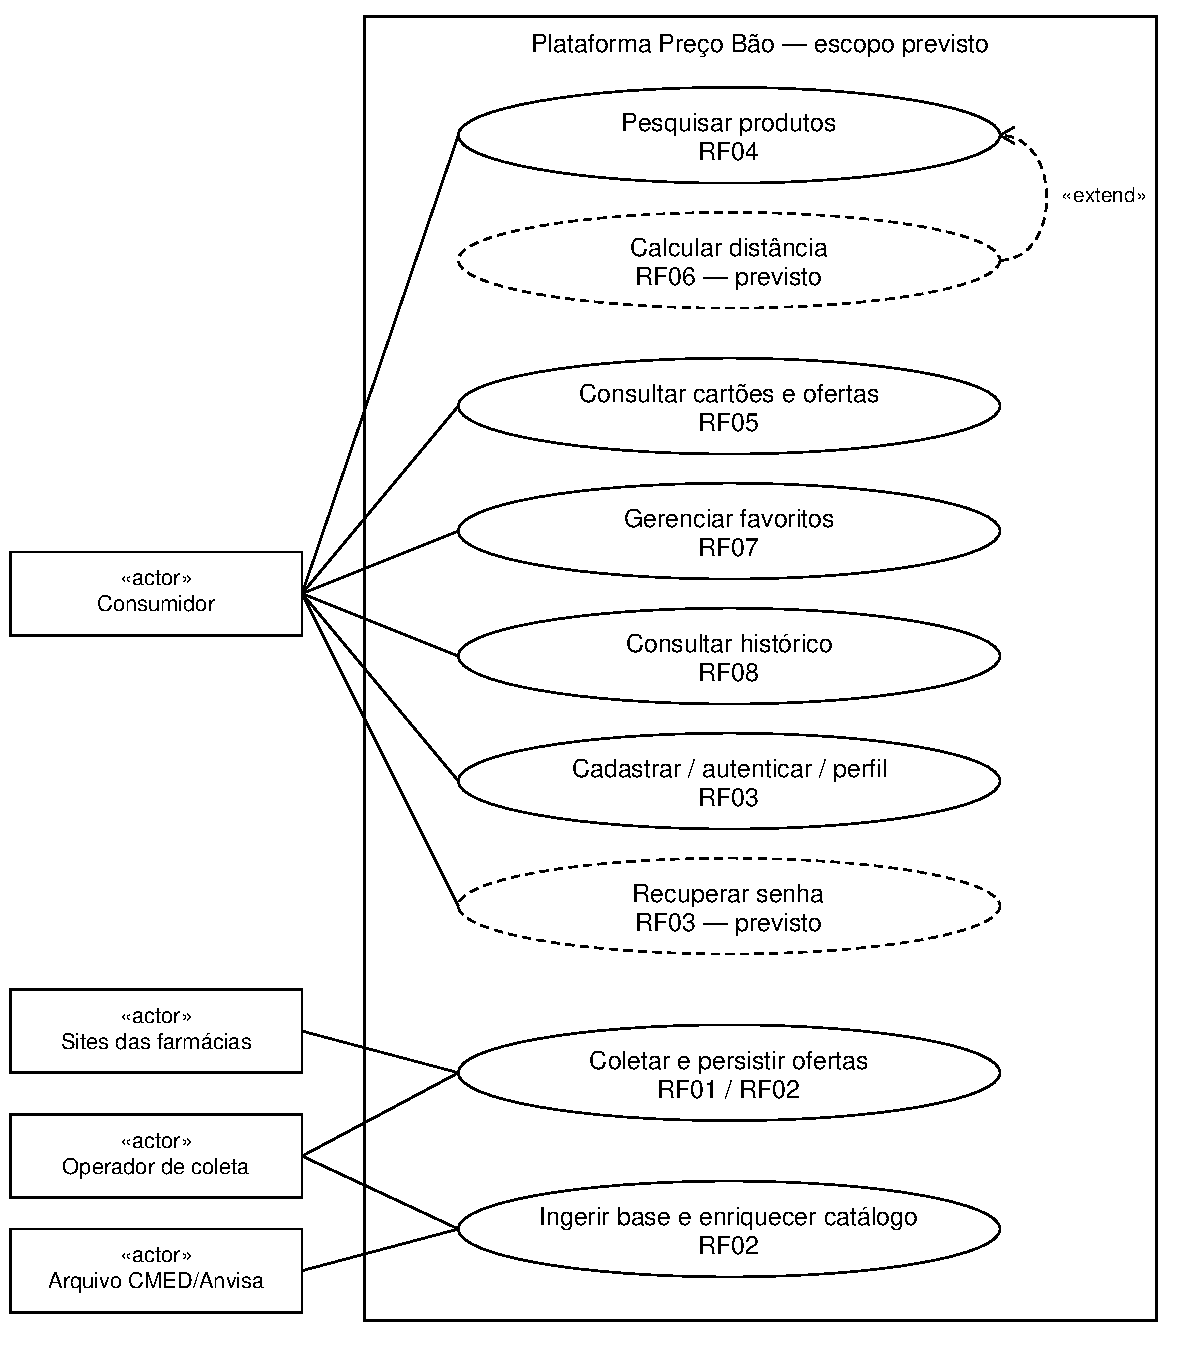
\includegraphics[width=\textwidth,height=0.74\textheight,keepaspectratio]{figures/diagrama-caso-de-uso.pdf}
\fonte{Elaboração a partir dos requisitos e das rotas do projeto (2026).}
\end{figure}

Autenticação é precondição para alterar perfil e gerenciar favoritos, sem exigir repetição do login a cada operação. Por isso esses casos não incluem automaticamente o caso de autenticar. O histórico implementado é público. O cálculo de distância é uma extensão prevista da pesquisa no ponto de apresentação/ordenação dos resultados, condicionada à permissão e à disponibilidade das coordenadas. Não há relação de inclusão artificial entre consulta e comparação, que podem ser realizadas separadamente.

\begin{description}
\item[UC01 -- Coletar ofertas (RF01).] Operador inicia a rotina; o coletor consulta a fonte e persiste observações. Falhas devem ser registradas e tratadas; continuidade entre fontes requer CT12.
\item[UC02 -- Enriquecer catálogo (RF02).] Operador fornece a base oficial; a aplicação cruza EANs. Ausência de correspondência não deve ser apresentada como validação regulatória concluída.
\item[UC03 -- Gerenciar conta (RF03).] Consumidor cadastra-se e autentica-se para acessar perfil. Dados inválidos devem ser rejeitados. Recuperação de senha é uma meta sem fluxo público demonstrado.
\item[UC04 -- Pesquisar ofertas (RF04/RF05).] Consumidor informa uma busca, consulta cartões e ofertas e escolhe ordenação. Sem resultado, a interface informa a ausência de itens.
\item[UC05 -- Calcular distância (RF06).] Extensão prevista de UC04, mediante permissão e coordenadas. Sem permissão, a pesquisa por preço deve continuar disponível.
\item[UC06 -- Gerenciar favoritos (RF07).] Conta ativa autenticada adiciona ou remove um produto; o vínculo é persistido para aquele usuário. Acesso sem autenticação deve ser recusado.
\item[UC07 -- Consultar histórico (RF08).] Consumidor consulta produto e período; a API retorna observações por farmácia e a interface apresenta a série. Uma série vazia não autoriza criar preços ou datas fictícios.
\end{description}

\subsection{Diagrama de Classes}

As três famílias distinguem coleta, contratos de dados e persistência. Os desenhos resumem membros relevantes; a enumeração completa das colunas está na Seção \ref{sec:dicionario}.

\subsubsection{Motor de \textit{scraping} (ETL)}

A classe abstrata real é \ident{BasePharmacyScraper}, em \file{app/scrapers/base.py}. Define \ident{extrair_catalogo} como método abstrato e oferece fila, processamento de lotes, workers e retentativas com backoff. \ident{AraujoScraper} e \ident{PachecoScraper} herdam essa classe. O módulo Indiana usa funções, incluindo \ident{extrair_todos_produtos}, \ident{adaptar_parser_rest} e \ident{salvar_no_banco}, sem herança da base. A Figura \ref{fig:diagrama_scraping} mantém essa distinção.

\begin{figure}[htb]
\centering\caption{Classes de coleta e módulo funcional Indiana}\label{fig:diagrama_scraping}
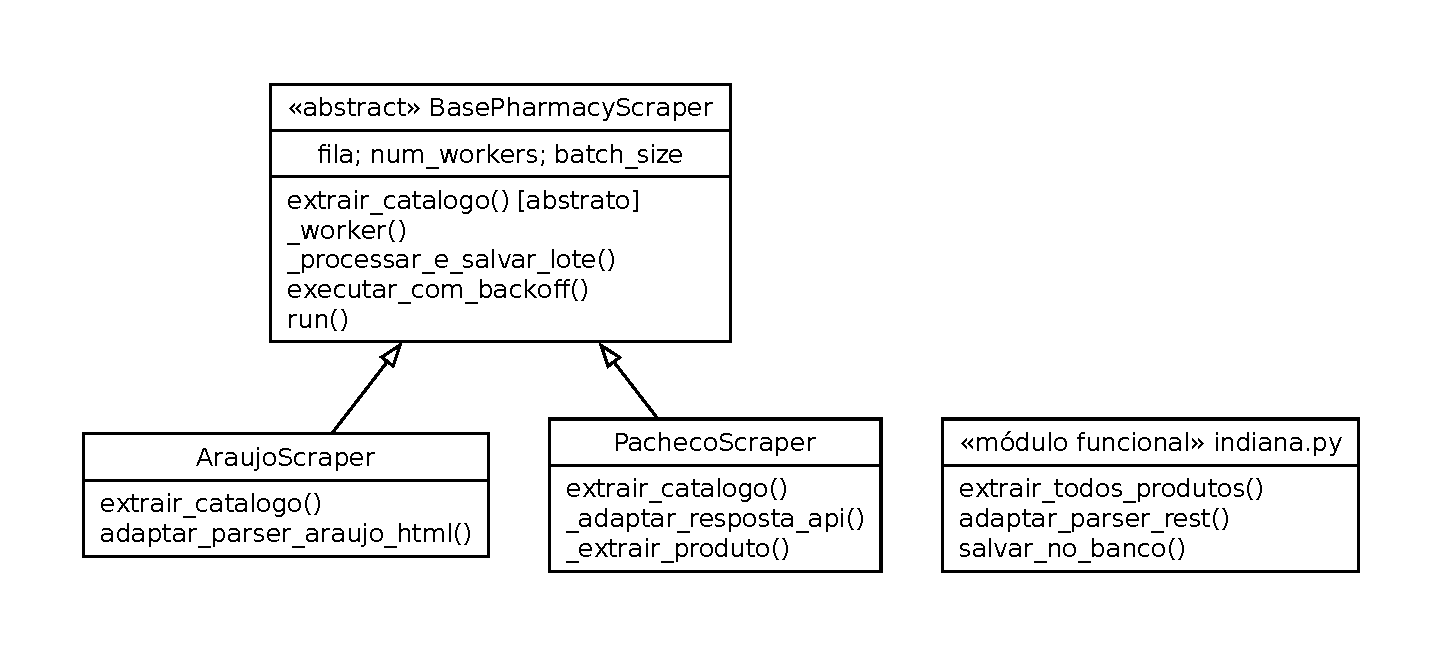
\includegraphics[width=\textwidth,height=0.48\textheight,keepaspectratio]{figures/diagrama-scraping.pdf}
\fonte{Elaboração a partir de \ident{app/scrapers/} (2026).}
\end{figure}

\subsubsection{\textit{Schemas} da API (Pydantic)}

\ident{UsuarioRead}, \ident{UsuarioCreate} e \ident{UsuarioUpdate} derivam, respectivamente, de \ident{BaseUser}, \ident{BaseUserCreate} e \ident{BaseUserUpdate} da biblioteca FastAPI Users. Leitura não inclui o hash; criação recebe o campo \ident{password} herdado. Não há \ident{UsuarioBase}, \ident{UsuarioOut} ou \ident{senha_clara} nos contratos consultados.

Catálogo e ofertas usam famílias próprias: \ident{CatalogoOut} deriva de \ident{CatalogoBaseSchema}; \ident{CatalogoComOfertasOut} agrega ofertas, sem herdar delas. \ident{OfertaOut} deriva de \ident{OfertaBaseSchema}. Para histórico coexistem contratos legados \ident{HistoricoBase/Out} e a resposta agregada \ident{MedicineHistoryResponse}, com séries e estatísticas. A Figura \ref{fig:diagrama_schemas} resume essas relações; linhas tracejadas sem triângulo representam referências a objetos, não herança.

\begin{figure}[htb]
\centering\caption{Famílias de contratos de dados da API}\label{fig:diagrama_schemas}
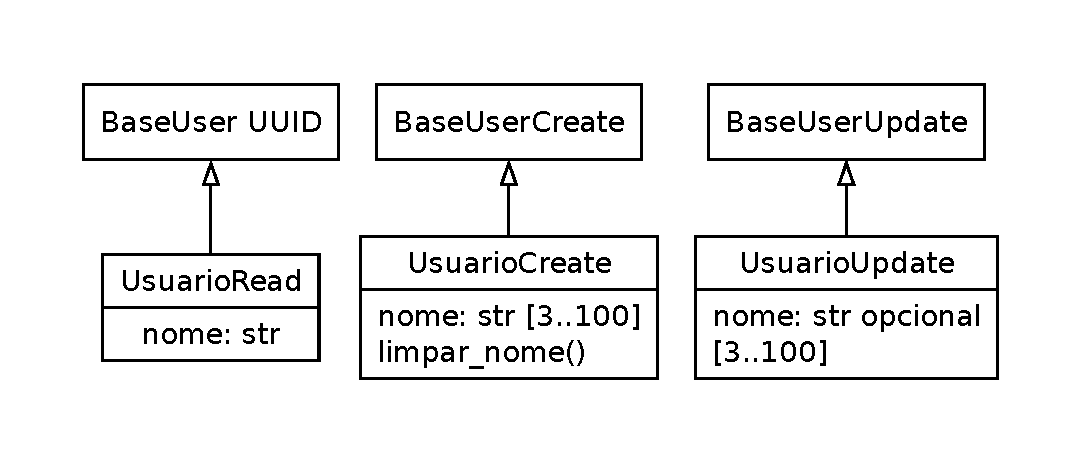
\includegraphics[width=0.95\textwidth,height=0.20\textheight,keepaspectratio]{figures/schemas-usuario.pdf}\par\medskip
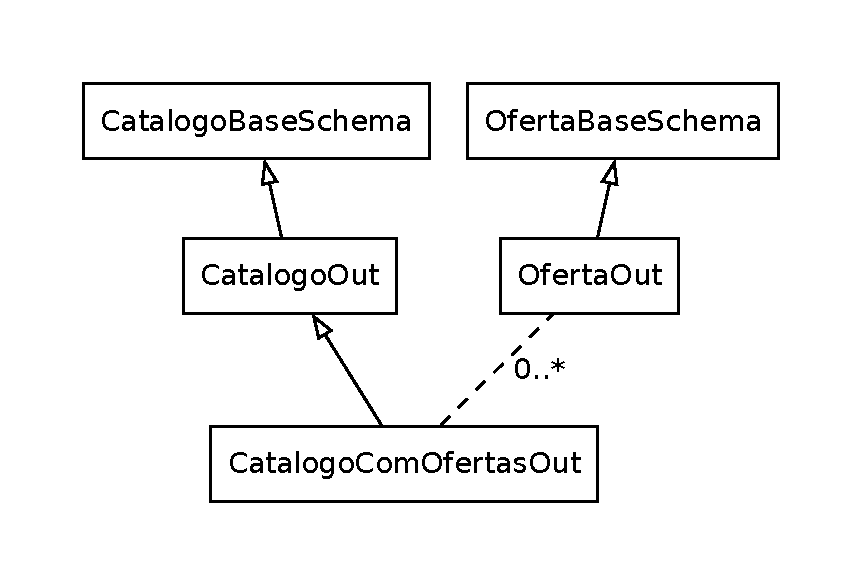
\includegraphics[width=0.95\textwidth,height=0.23\textheight,keepaspectratio]{figures/schemas-catalogo.pdf}\par\medskip
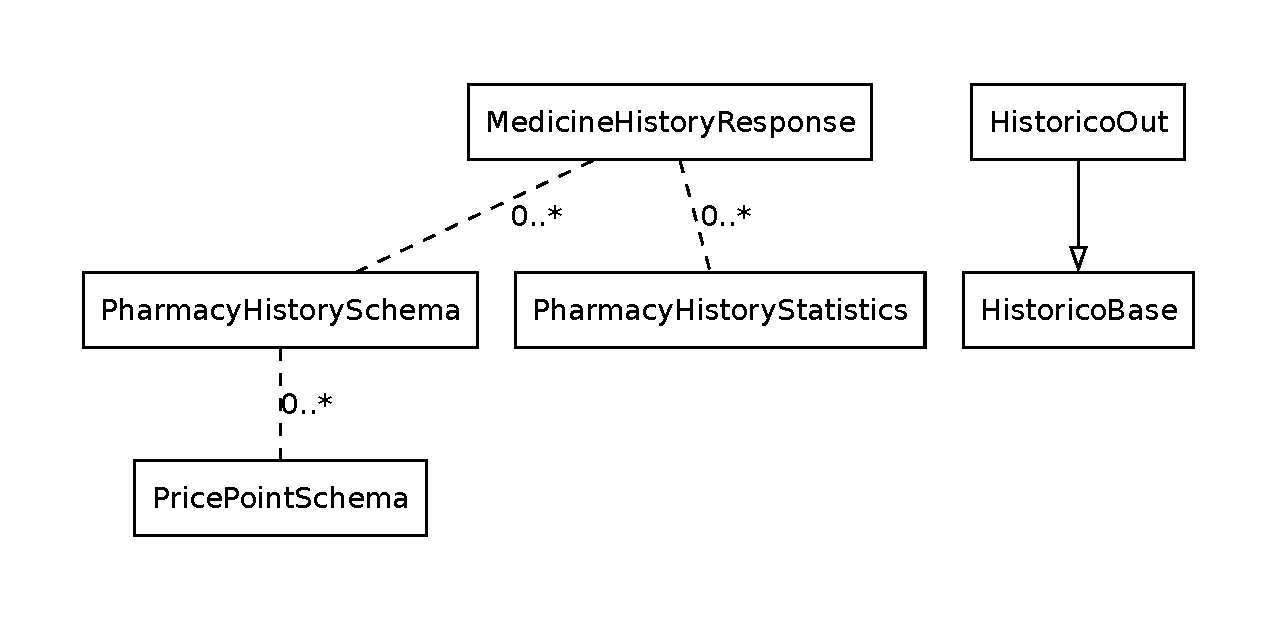
\includegraphics[width=0.95\textwidth,height=0.25\textheight,keepaspectratio]{figures/schemas-historico.pdf}
\fonte{Elaboração a partir de \ident{app/schemas/} (2026).}
\end{figure}

\subsubsection{Mapeamento objeto-relacional (SQLAlchemy ORM)}

\ident{Base} gerencia metadados e convenções; não injeta automaticamente colunas de identificação ou datas em todas as entidades. \ident{Usuario} herda UUID, e-mail, \ident{hashed_password} e indicadores de conta de \ident{SQLAlchemyBaseUserTableUUID}, acrescentando \ident{nome}. Não possui \ident{criado_em} no modelo consultado.

\ident{CatalogoBase} separa a identidade do produto das ofertas comerciais de \ident{OfertaFarmacia}; inclui classificação e metadados de imagem, que podem evoluir. \ident{Farmacia} mantém dados do estabelecimento. \ident{HistoricoPreco} vincula produto e farmácia e, opcionalmente, a oferta observada. \ident{AnvisaMedicamento} é uma base local de enriquecimento por EAN; não existe FK entre ela e o catálogo.

Favoritos são duas tabelas associativas, \ident{usuario_medicamento_favorito} e \ident{usuario_farmacia_favorita}, com chaves primárias compostas; não existe classe persistente genérica \ident{Favorito}. A Figura \ref{fig:diagrama_orm} distingue as classes das associações do tipo \ident{Table}.

\begin{figure}[htb]
\centering\caption{Visão resumida das classes ORM e associações}\label{fig:diagrama_orm}
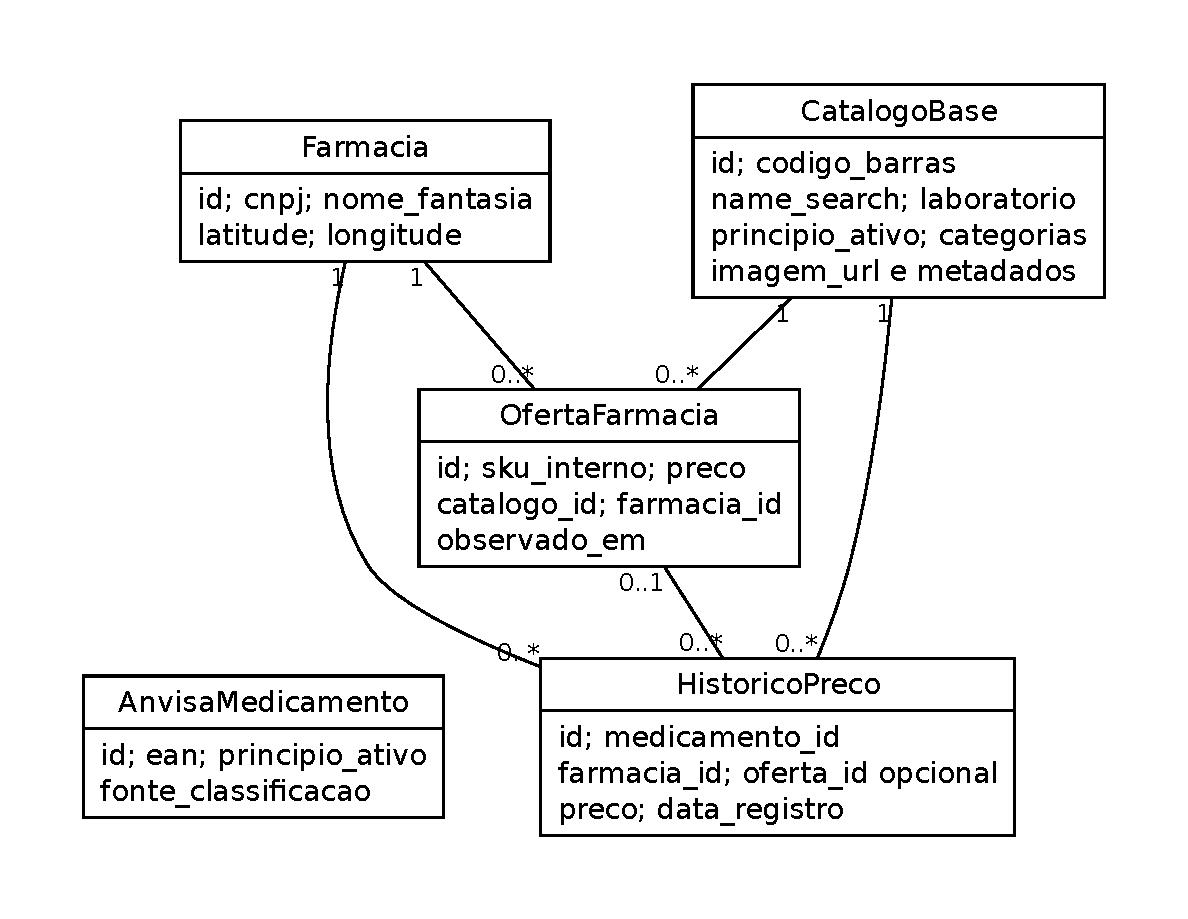
\includegraphics[width=\textwidth,height=0.40\textheight,keepaspectratio]{figures/orm-dominio.pdf}\par\medskip
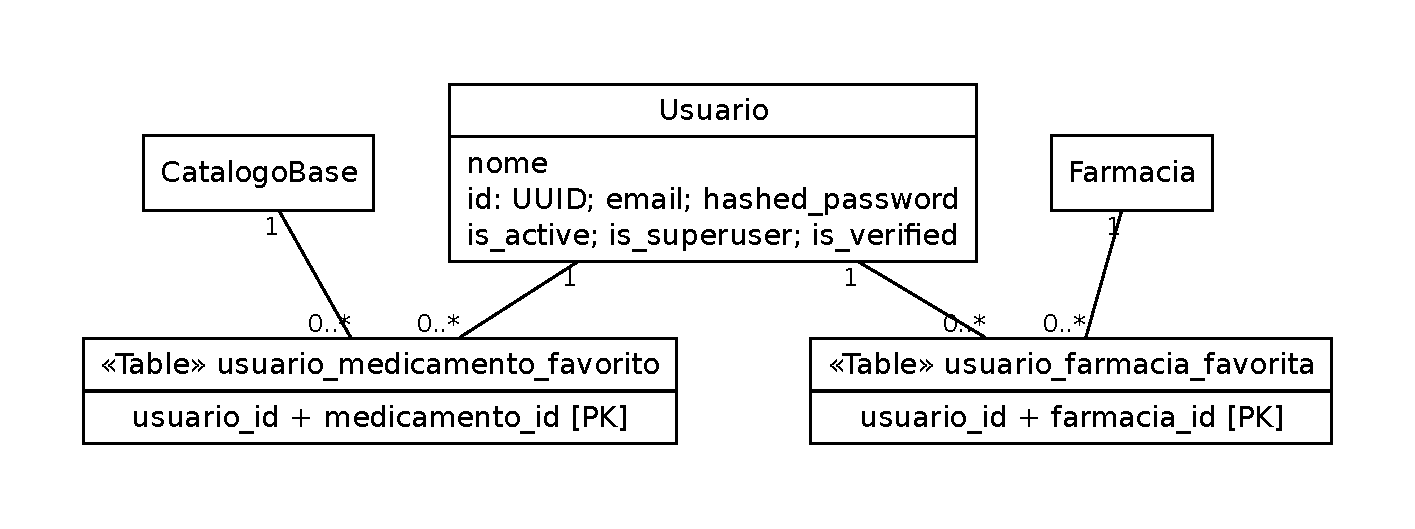
\includegraphics[width=\textwidth,height=0.28\textheight,keepaspectratio]{figures/orm-usuarios.pdf}
\fonte{Elaboração a partir de \ident{app/models/} (2026).}
\end{figure}

\section{Projeto de banco de dados}\label{sec:banco}

O esquema documentado é o dos metadados ORM do checkout examinado, compilados para PostgreSQL e confrontados com as migrações até \ident{e4902ba81c6d}. Isso não certifica a versão de um banco em execução. A Figura \ref{fig:der} é o diagrama entidade-relacionamento (DER), com chaves e cardinalidades; o dicionário apresenta todas as colunas.

\begin{sidewaysfigure}[p]
\centering\caption{DER do esquema ORM para PostgreSQL}\label{fig:der}
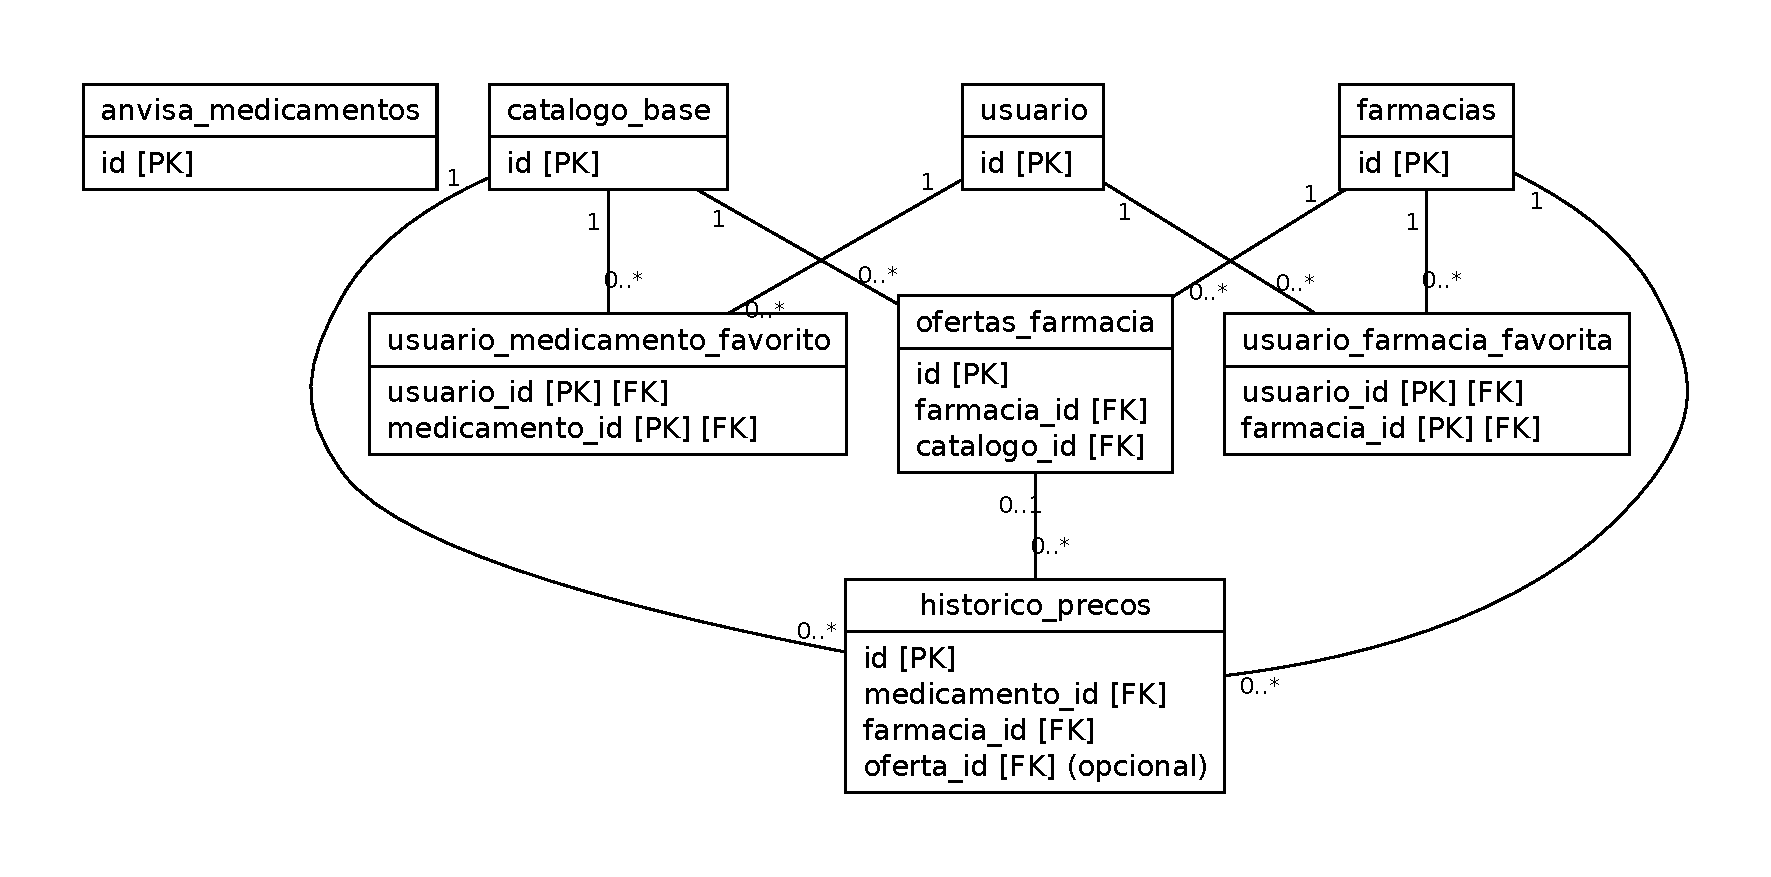
\includegraphics[width=\textheight,height=0.75\textwidth,keepaspectratio]{figures/der.pdf}
\fonte{Metadados SQLAlchemy em \ident{app/models/} (2026).}
\end{sidewaysfigure}

Cada oferta pertence a um produto e a uma farmácia; cada um pode ter zero ou muitas ofertas. Cada observação histórica pertence a um produto e a uma farmácia e pode referenciar zero ou uma oferta; uma oferta pode ter muitas observações. As associações de favoritos resolvem relações muitos-para-muitos com o usuário. Cada par de chaves é único pela PK composta, com exclusão em cascata no banco para as duas FKs dessas associações. Cascatas de relacionamento no ORM não devem ser confundidas com \ident{ON DELETE} em outras FKs.

As entidades podem ser localizadas diretamente nas descrições: \ident{anvisa_medicamentos} (\ref{dic:anvisa_medicamentos}), \ident{catalogo_base} (\ref{dic:catalogo_base}), \ident{farmacias} (\ref{dic:farmacias}), \ident{usuario} (\ref{dic:usuario}), \ident{ofertas_farmacia} (\ref{dic:ofertas_farmacia}), \ident{historico_precos} (\ref{dic:historico_precos}) e as associações de favoritos (\ref{dic:usuario_farmacia_favorita} e \ref{dic:usuario_medicamento_favorito}).

\subsection{Restrições e divergências entre fontes}

As chaves únicas incluem CNPJ, código de barras quando presente, EAN da base Anvisa, URL de origem da oferta e e-mail. O SKU não é globalmente único. O esquema não declara restrições CHECK para preço positivo ou limites de coordenadas; validações de aplicação não equivalem a restrições no banco. Campos oficiais anuláveis preservam a distinção entre classificação desconhecida e falsa.

A migração \ident{1de74e4279f7} define padrão SQL de array vazio para categorias; o modelo define \texttt{default=list} em Python. A migração \ident{3a72d8ce1f40} cria índice composto de histórico por medicamento, farmácia e data, ausente da declaração de índices ORM. A representação ORM é usada no DER e no dicionário, sem omitir essas diferenças. O dicionário inclui padrões SQL declarados no ORM; os padrões apenas Python não se aplicam a inserções SQL diretas. Não se comprova retenção por 12 meses pela existência de datas ou filtros temporais.

% Gerado por scripts/gerar_artefatos.py; não editar manualmente.
\begingroup\def\LTcaptype{quadro}
\subsection{Dicionário de dados}\label{sec:dicionario}
A descrição representa os metadados ORM do checkout revisado, compilados para PostgreSQL. Nulo indica se a coluna admite SQL NULL; PK é chave primária e FK é chave estrangeira. Padrões Python são aplicados pela aplicação e não equivalem a padrões SQL. Não há consulta a um banco em execução.
\subsubsection{anvisa\_medicamentos}\label{dic:anvisa_medicamentos}
Base local de consulta oficial; cruzamento por EAN na aplicação, sem FK para o catálogo.
\begingroup\footnotesize\setlength{\tabcolsep}{3pt}
\begin{longtable}{|>{\raggedright\arraybackslash}p{0.27\textwidth}|>{\raggedright\arraybackslash}p{0.22\textwidth}|>{\raggedright\arraybackslash}p{0.43\textwidth}|}
\caption{Dicionário: anvisa\_medicamentos}\label{qua:dic-anvisa_medicamentos}\\\hline
\textbf{Coluna} & \textbf{Tipo / nulo} & \textbf{Descrição e restrições} \\\hline\endfirsthead
\multicolumn{3}{l}{Quadro \thequadro\ -- continuação}\\\hline
\textbf{Coluna} & \textbf{Tipo / nulo} & \textbf{Descrição e restrições} \\\hline\endhead
\multicolumn{3}{r}{Continua na próxima página.}\\\endfoot
\multicolumn{3}{l}{Fonte: metadados ORM do projeto (2026).}\\\endlastfoot
\ident{id} & INTEGER / não & Identificador do registro. PK. \\\hline
\ident{ean} & VARCHAR(14) / não & Código EAN da base oficial. único. \\\hline
\ident{principio_ativo} & VARCHAR / sim & Princípio ativo informado pela fonte. \\\hline
\ident{laboratorio} & VARCHAR / sim & Laboratório informado. \\\hline
\ident{tarja} & VARCHAR / sim & Classificação de tarja informada. \\\hline
\ident{registro_anvisa} & VARCHAR(20) / sim & Identificador de registro na Anvisa. \\\hline
\ident{categoria_regulatoria} & VARCHAR(40) / sim & Categoria regulatória identificada na fonte. \\\hline
\ident{status_registro} & VARCHAR(40) / sim & Situação do registro na fonte. \\\hline
\ident{referencia_anvisa} & BOOLEAN / sim & Indicador de medicamento de referência. \\\hline
\ident{exige_receita_confirmada} & BOOLEAN / sim & Exigência de receita confirmada na fonte. \\\hline
\ident{controle_especial} & BOOLEAN / sim & Indicador de controle especial. \\\hline
\ident{fonte_classificacao} & VARCHAR(120) / sim & Procedência da classificação oficial. \\\hline
\ident{atualizado_fonte_em} & DATE / sim & Data de atualização informada pela fonte. \\\hline
\end{longtable}\endgroup
\subsubsection{catalogo\_base}\label{dic:catalogo_base}
Identidade e classificação dos produtos e referências de imagens.
\begingroup\footnotesize\setlength{\tabcolsep}{3pt}
\begin{longtable}{|>{\raggedright\arraybackslash}p{0.27\textwidth}|>{\raggedright\arraybackslash}p{0.22\textwidth}|>{\raggedright\arraybackslash}p{0.43\textwidth}|}
\caption{Dicionário: catalogo\_base}\label{qua:dic-catalogo_base}\\\hline
\textbf{Coluna} & \textbf{Tipo / nulo} & \textbf{Descrição e restrições} \\\hline\endfirsthead
\multicolumn{3}{l}{Quadro \thequadro\ -- continuação}\\\hline
\textbf{Coluna} & \textbf{Tipo / nulo} & \textbf{Descrição e restrições} \\\hline\endhead
\multicolumn{3}{r}{Continua na próxima página.}\\\endfoot
\multicolumn{3}{l}{Fonte: metadados ORM do projeto (2026).}\\\endlastfoot
\ident{id} & INTEGER / não & Identificador do registro. PK. \\\hline
\ident{codigo_barras} & VARCHAR(14) / sim & EAN/GTIN do item; pode estar ausente. único. \\\hline
\ident{name_search} & VARCHAR(150) / não & Nome utilizado nas pesquisas. \\\hline
\ident{principio_ativo} & VARCHAR(500) / não & Princípio ativo informado pela fonte. padrão Python: \ident{Não informado}. \\\hline
\ident{laboratorio} & VARCHAR(100) / não & Laboratório informado. padrão Python: \ident{Não informado}. \\\hline
\ident{exige_receita} & BOOLEAN / não & Indicador legado de exigência de receita. padrão Python: \ident{False}. \\\hline
\ident{categoria_regulatoria} & VARCHAR(40) / sim & Categoria regulatória identificada na fonte. \\\hline
\ident{referencia_anvisa} & BOOLEAN / sim & Indicador de medicamento de referência. \\\hline
\ident{exige_receita_confirmada} & BOOLEAN / sim & Exigência de receita confirmada na fonte. \\\hline
\ident{controle_especial} & BOOLEAN / sim & Indicador de controle especial. \\\hline
\ident{classificacao_fonte} & VARCHAR(80) / sim & Procedência da classificação. \\\hline
\ident{categorias} & VARCHAR[] / não & Lista de categorias do catálogo. padrão Python: \ident{list}. \\\hline
\ident{imagem_url} & VARCHAR(500) / sim & Referência externa da imagem; não armazena a fotografia. \\\hline
\ident{imagem_fonte} & VARCHAR(40) / sim & Origem da referência de imagem. \\\hline
\ident{imagem_sku_origem} & VARCHAR(80) / sim & SKU que sustenta a associação da imagem. \\\hline
\ident{imagem_ean} & VARCHAR(14) / sim & EAN usado como evidência da imagem. \\\hline
\ident{imagem_match} & VARCHAR(24) / sim & Tipo de correspondência de identidade. \\\hline
\ident{imagem_status} & VARCHAR(20) / sim & Estado de verificação da referência. \\\hline
\ident{imagem_atualizada_em} & timestamp com fuso / sim & Instante de alteração da referência. \\\hline
\ident{imagem_verificada_em} & timestamp com fuso / sim & Última validação bem-sucedida. \\\hline
\ident{imagem_ultima_verificacao_em} & timestamp com fuso / sim & Instante da última tentativa de validação. \\\hline
\ident{imagem_falhas_consecutivas} & INTEGER / não & Contador de falhas seguidas. padrão SQL: \ident{0}; padrão Python: \ident{0}. \\\hline
\ident{imagem_ultima_falha} & TEXT / sim & Descrição da falha recente. \\\hline
\ident{imagem_motivo_rejeicao} & TEXT / sim & Motivo de rejeição da referência. \\\hline
\ident{criado_em} & timestamp com fuso / não & Instante de criação. padrão SQL: \ident{now()}. \\\hline
\ident{atualizado_em} & timestamp com fuso / sim & Instante da última atualização; ORM preenche ao alterar. \\\hline
\end{longtable}\endgroup
\subsubsection{farmacias}\label{dic:farmacias}
Cadastro dos estabelecimentos e coordenadas.
\begingroup\footnotesize\setlength{\tabcolsep}{3pt}
\begin{longtable}{|>{\raggedright\arraybackslash}p{0.27\textwidth}|>{\raggedright\arraybackslash}p{0.22\textwidth}|>{\raggedright\arraybackslash}p{0.43\textwidth}|}
\caption{Dicionário: farmacias}\label{qua:dic-farmacias}\\\hline
\textbf{Coluna} & \textbf{Tipo / nulo} & \textbf{Descrição e restrições} \\\hline\endfirsthead
\multicolumn{3}{l}{Quadro \thequadro\ -- continuação}\\\hline
\textbf{Coluna} & \textbf{Tipo / nulo} & \textbf{Descrição e restrições} \\\hline\endhead
\multicolumn{3}{r}{Continua na próxima página.}\\\endfoot
\multicolumn{3}{l}{Fonte: metadados ORM do projeto (2026).}\\\endlastfoot
\ident{id} & INTEGER / não & Identificador do registro. PK. \\\hline
\ident{cnpj} & VARCHAR(14) / não & CNPJ da farmácia. único. \\\hline
\ident{razao_social} & VARCHAR(150) / não & Razão social cadastrada. \\\hline
\ident{nome_fantasia} & VARCHAR(100) / não & Nome comercial da farmácia. \\\hline
\ident{telefone} & VARCHAR(20) / sim & Contato telefônico. \\\hline
\ident{endereco_completo} & VARCHAR(255) / não & Endereço cadastrado. \\\hline
\ident{latitude} & NUMERIC(9, 6) / sim & Latitude do estabelecimento. \\\hline
\ident{longitude} & NUMERIC(10, 6) / sim & Longitude do estabelecimento. \\\hline
\ident{criado_em} & timestamp com fuso / não & Instante de criação. padrão SQL: \ident{now()}. \\\hline
\ident{atualizado_em} & timestamp com fuso / sim & Instante da última atualização; ORM preenche ao alterar. \\\hline
\end{longtable}\endgroup
\subsubsection{usuario}\label{dic:usuario}
Conta; nome é declarado localmente e os demais campos são herdados de SQLAlchemyBaseUserTableUUID.
\begingroup\footnotesize\setlength{\tabcolsep}{3pt}
\begin{longtable}{|>{\raggedright\arraybackslash}p{0.27\textwidth}|>{\raggedright\arraybackslash}p{0.22\textwidth}|>{\raggedright\arraybackslash}p{0.43\textwidth}|}
\caption{Dicionário: usuario}\label{qua:dic-usuario}\\\hline
\textbf{Coluna} & \textbf{Tipo / nulo} & \textbf{Descrição e restrições} \\\hline\endfirsthead
\multicolumn{3}{l}{Quadro \thequadro\ -- continuação}\\\hline
\textbf{Coluna} & \textbf{Tipo / nulo} & \textbf{Descrição e restrições} \\\hline\endhead
\multicolumn{3}{r}{Continua na próxima página.}\\\endfoot
\multicolumn{3}{l}{Fonte: metadados ORM do projeto (2026).}\\\endlastfoot
\ident{nome} & VARCHAR(100) / não & Nome cadastrado do usuário. \\\hline
\ident{id} & UUID / não & Identificador do registro. PK; padrão Python: \ident{uuid4}. \\\hline
\ident{email} & VARCHAR(320) / não & E-mail de autenticação. único. \\\hline
\ident{hashed_password} & VARCHAR(1024) / não & Resumo criptográfico da senha; nunca resposta pública. \\\hline
\ident{is_active} & BOOLEAN / não & Indicador de conta ativa. padrão Python: \ident{True}. \\\hline
\ident{is_superuser} & BOOLEAN / não & Indicador de privilégio administrativo. padrão Python: \ident{False}. \\\hline
\ident{is_verified} & BOOLEAN / não & Indicador de verificação da conta. padrão Python: \ident{False}. \\\hline
\end{longtable}\endgroup
\subsubsection{ofertas\_farmacia}\label{dic:ofertas_farmacia}
Ocorrências comerciais de produtos em farmácias.
\begingroup\footnotesize\setlength{\tabcolsep}{3pt}
\begin{longtable}{|>{\raggedright\arraybackslash}p{0.27\textwidth}|>{\raggedright\arraybackslash}p{0.22\textwidth}|>{\raggedright\arraybackslash}p{0.43\textwidth}|}
\caption{Dicionário: ofertas\_farmacia}\label{qua:dic-ofertas_farmacia}\\\hline
\textbf{Coluna} & \textbf{Tipo / nulo} & \textbf{Descrição e restrições} \\\hline\endfirsthead
\multicolumn{3}{l}{Quadro \thequadro\ -- continuação}\\\hline
\textbf{Coluna} & \textbf{Tipo / nulo} & \textbf{Descrição e restrições} \\\hline\endhead
\multicolumn{3}{r}{Continua na próxima página.}\\\endfoot
\multicolumn{3}{l}{Fonte: metadados ORM do projeto (2026).}\\\endlastfoot
\ident{id} & INTEGER / não & Identificador do registro. PK. \\\hline
\ident{sku_interno} & VARCHAR(50) / não & Identificador do produto na farmácia; não é EAN. \\\hline
\ident{preco} & NUMERIC(10, 2) / não & Preço observado, com duas casas decimais. \\\hline
\ident{quantidade_estoque} & INTEGER / não & Quantidade informada pela coleta, sem garantia de estoque físico. padrão Python: \ident{0}. \\\hline
\ident{disponivel} & BOOLEAN / não & Disponibilidade observada na fonte. padrão Python: \ident{True}. \\\hline
\ident{url_origem} & VARCHAR(500) / não & Página pública de origem da oferta. único. \\\hline
\ident{imagem_url} & VARCHAR(500) / sim & Referência externa da imagem; não armazena a fotografia. \\\hline
\ident{criado_em} & timestamp com fuso / não & Instante de criação. padrão SQL: \ident{now()}. \\\hline
\ident{atualizado_em} & timestamp com fuso / sim & Instante da última atualização; ORM preenche ao alterar. \\\hline
\ident{observado_em} & timestamp com fuso / sim & Instante da observação da oferta. \\\hline
\ident{farmacia_id} & INTEGER / não & Vínculo com a farmácia. FK \ident{farmacias.id}. \\\hline
\ident{catalogo_id} & INTEGER / não & Vínculo com o item do catálogo. FK \ident{catalogo_base.id}. \\\hline
\end{longtable}\endgroup
\subsubsection{usuario\_farmacia\_favorita}\label{dic:usuario_farmacia_favorita}
Associação de usuários com farmácias favoritas, sem coluna id própria.
\begingroup\footnotesize\setlength{\tabcolsep}{3pt}
\begin{longtable}{|>{\raggedright\arraybackslash}p{0.27\textwidth}|>{\raggedright\arraybackslash}p{0.22\textwidth}|>{\raggedright\arraybackslash}p{0.43\textwidth}|}
\caption{Dicionário: usuario\_farmacia\_favorita}\label{qua:dic-usuario_farmacia_favorita}\\\hline
\textbf{Coluna} & \textbf{Tipo / nulo} & \textbf{Descrição e restrições} \\\hline\endfirsthead
\multicolumn{3}{l}{Quadro \thequadro\ -- continuação}\\\hline
\textbf{Coluna} & \textbf{Tipo / nulo} & \textbf{Descrição e restrições} \\\hline\endhead
\multicolumn{3}{r}{Continua na próxima página.}\\\endfoot
\multicolumn{3}{l}{Fonte: metadados ORM do projeto (2026).}\\\endlastfoot
\ident{usuario_id} & UUID / não & Vínculo com o usuário. PK composta; FK \ident{usuario.id}. ON DELETE CASCADE. \\\hline
\ident{farmacia_id} & INTEGER / não & Vínculo com a farmácia. PK composta; FK \ident{farmacias.id}. ON DELETE CASCADE. \\\hline
\end{longtable}\endgroup
\subsubsection{usuario\_medicamento\_favorito}\label{dic:usuario_medicamento_favorito}
Associação de usuários com medicamentos favoritos, sem coluna id própria.
\begingroup\footnotesize\setlength{\tabcolsep}{3pt}
\begin{longtable}{|>{\raggedright\arraybackslash}p{0.27\textwidth}|>{\raggedright\arraybackslash}p{0.22\textwidth}|>{\raggedright\arraybackslash}p{0.43\textwidth}|}
\caption{Dicionário: usuario\_medicamento\_favorito}\label{qua:dic-usuario_medicamento_favorito}\\\hline
\textbf{Coluna} & \textbf{Tipo / nulo} & \textbf{Descrição e restrições} \\\hline\endfirsthead
\multicolumn{3}{l}{Quadro \thequadro\ -- continuação}\\\hline
\textbf{Coluna} & \textbf{Tipo / nulo} & \textbf{Descrição e restrições} \\\hline\endhead
\multicolumn{3}{r}{Continua na próxima página.}\\\endfoot
\multicolumn{3}{l}{Fonte: metadados ORM do projeto (2026).}\\\endlastfoot
\ident{usuario_id} & UUID / não & Vínculo com o usuário. PK composta; FK \ident{usuario.id}. ON DELETE CASCADE. \\\hline
\ident{medicamento_id} & INTEGER / não & Vínculo com o item do catálogo. PK composta; FK \ident{catalogo_base.id}. ON DELETE CASCADE. \\\hline
\end{longtable}\endgroup
\subsubsection{historico\_precos}\label{dic:historico_precos}
Observações de preço vinculadas a produto e farmácia.
\begingroup\footnotesize\setlength{\tabcolsep}{3pt}
\begin{longtable}{|>{\raggedright\arraybackslash}p{0.27\textwidth}|>{\raggedright\arraybackslash}p{0.22\textwidth}|>{\raggedright\arraybackslash}p{0.43\textwidth}|}
\caption{Dicionário: historico\_precos}\label{qua:dic-historico_precos}\\\hline
\textbf{Coluna} & \textbf{Tipo / nulo} & \textbf{Descrição e restrições} \\\hline\endfirsthead
\multicolumn{3}{l}{Quadro \thequadro\ -- continuação}\\\hline
\textbf{Coluna} & \textbf{Tipo / nulo} & \textbf{Descrição e restrições} \\\hline\endhead
\multicolumn{3}{r}{Continua na próxima página.}\\\endfoot
\multicolumn{3}{l}{Fonte: metadados ORM do projeto (2026).}\\\endlastfoot
\ident{id} & INTEGER / não & Identificador do registro. PK. \\\hline
\ident{medicamento_id} & INTEGER / não & Vínculo com o item do catálogo. FK \ident{catalogo_base.id}. \\\hline
\ident{farmacia_id} & INTEGER / não & Vínculo com a farmácia. FK \ident{farmacias.id}. \\\hline
\ident{oferta_id} & INTEGER / sim & Oferta associada à observação; registros legados podem não ter vínculo. FK \ident{ofertas_farmacia.id}. \\\hline
\ident{origem} & VARCHAR(40) / sim & Origem da observação de preço. \\\hline
\ident{preco} & NUMERIC(10, 2) / não & Preço observado, com duas casas decimais. \\\hline
\ident{disponivel} & BOOLEAN / sim & Disponibilidade observada na fonte. \\\hline
\ident{data_registro} & timestamp sem fuso / não & Instante do registro histórico, sem fuso no banco. padrão SQL: \ident{now()}. \\\hline
\end{longtable}\endgroup
\endgroup


\section{Projeto de interfaces e navegação}\label{sec:interfaces}

A imagem preservada é um protótipo de baixa fidelidade, assim identificado no próprio arquivo. Não é captura da aplicação atual. Os metadados do PNG indicam exportação pelo Figma. Não foi localizado o projeto editável nem registro de validação com usuários. A Figura \ref{fig:prototipo_telas} mantém a composição original; as Figuras \ref{fig:prototipo_conta_inicio}, \ref{fig:prototipo_detalhe_busca} e \ref{fig:prototipo_historico} ampliam seus rótulos.

\begin{figure}[htb]
\centering\caption{Visão geral do protótipo de baixa fidelidade}\label{fig:prototipo_telas}
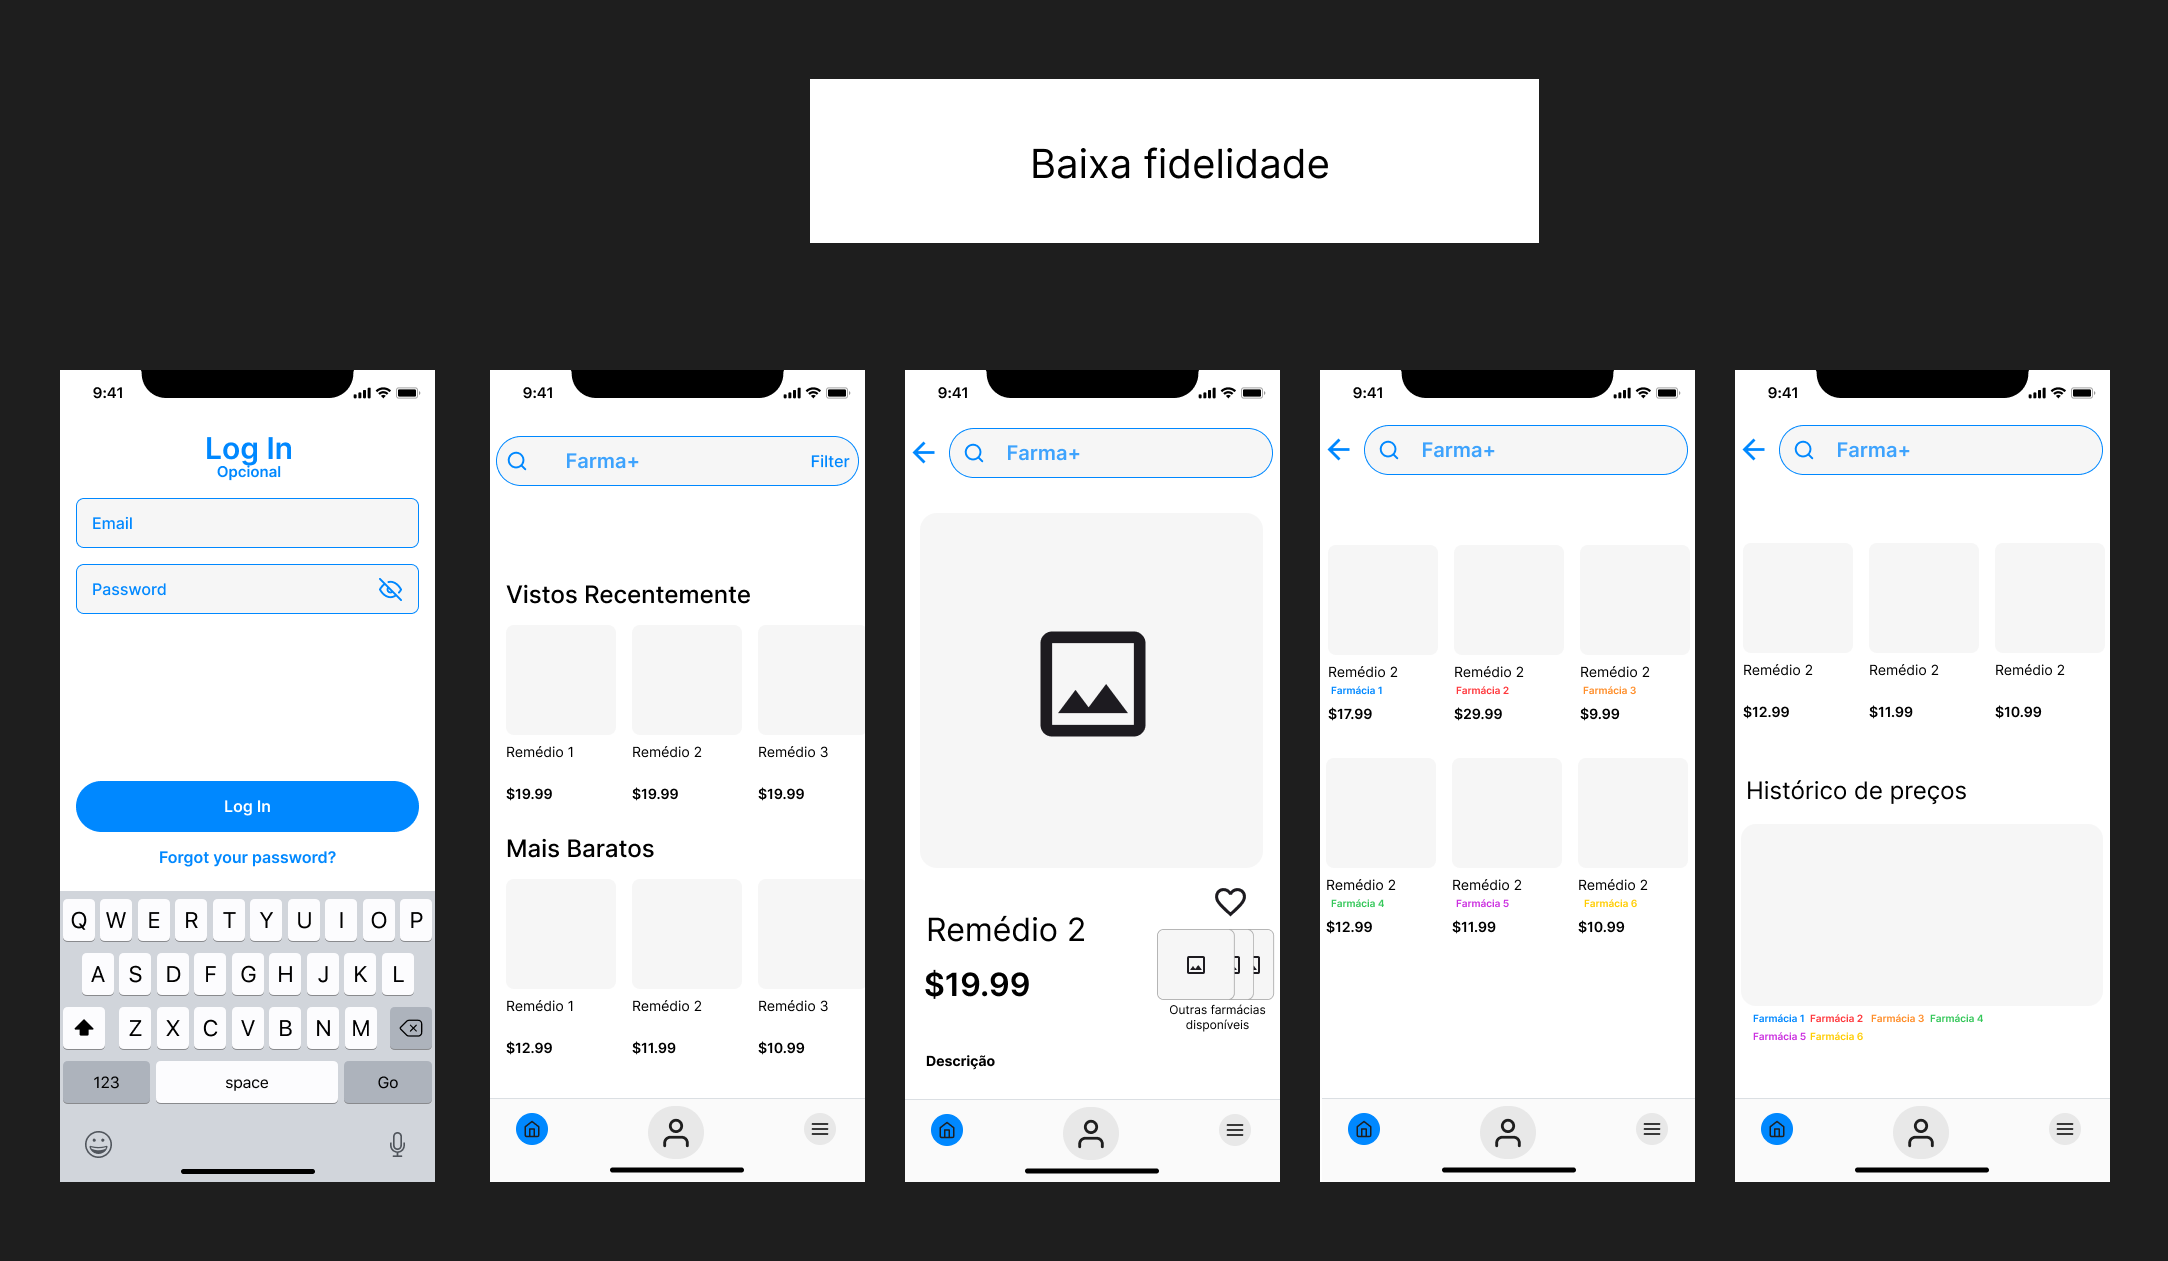
\includegraphics[width=\textwidth]{figures/prototipo-telas.png}
\fonte{Protótipo preservado no repositório, arquivo \ident{prototipo-telas.png}.}
\end{figure}

\begin{figure}[p]
\centering\caption{Ampliação do protótipo: login e início}\label{fig:prototipo_conta_inicio}
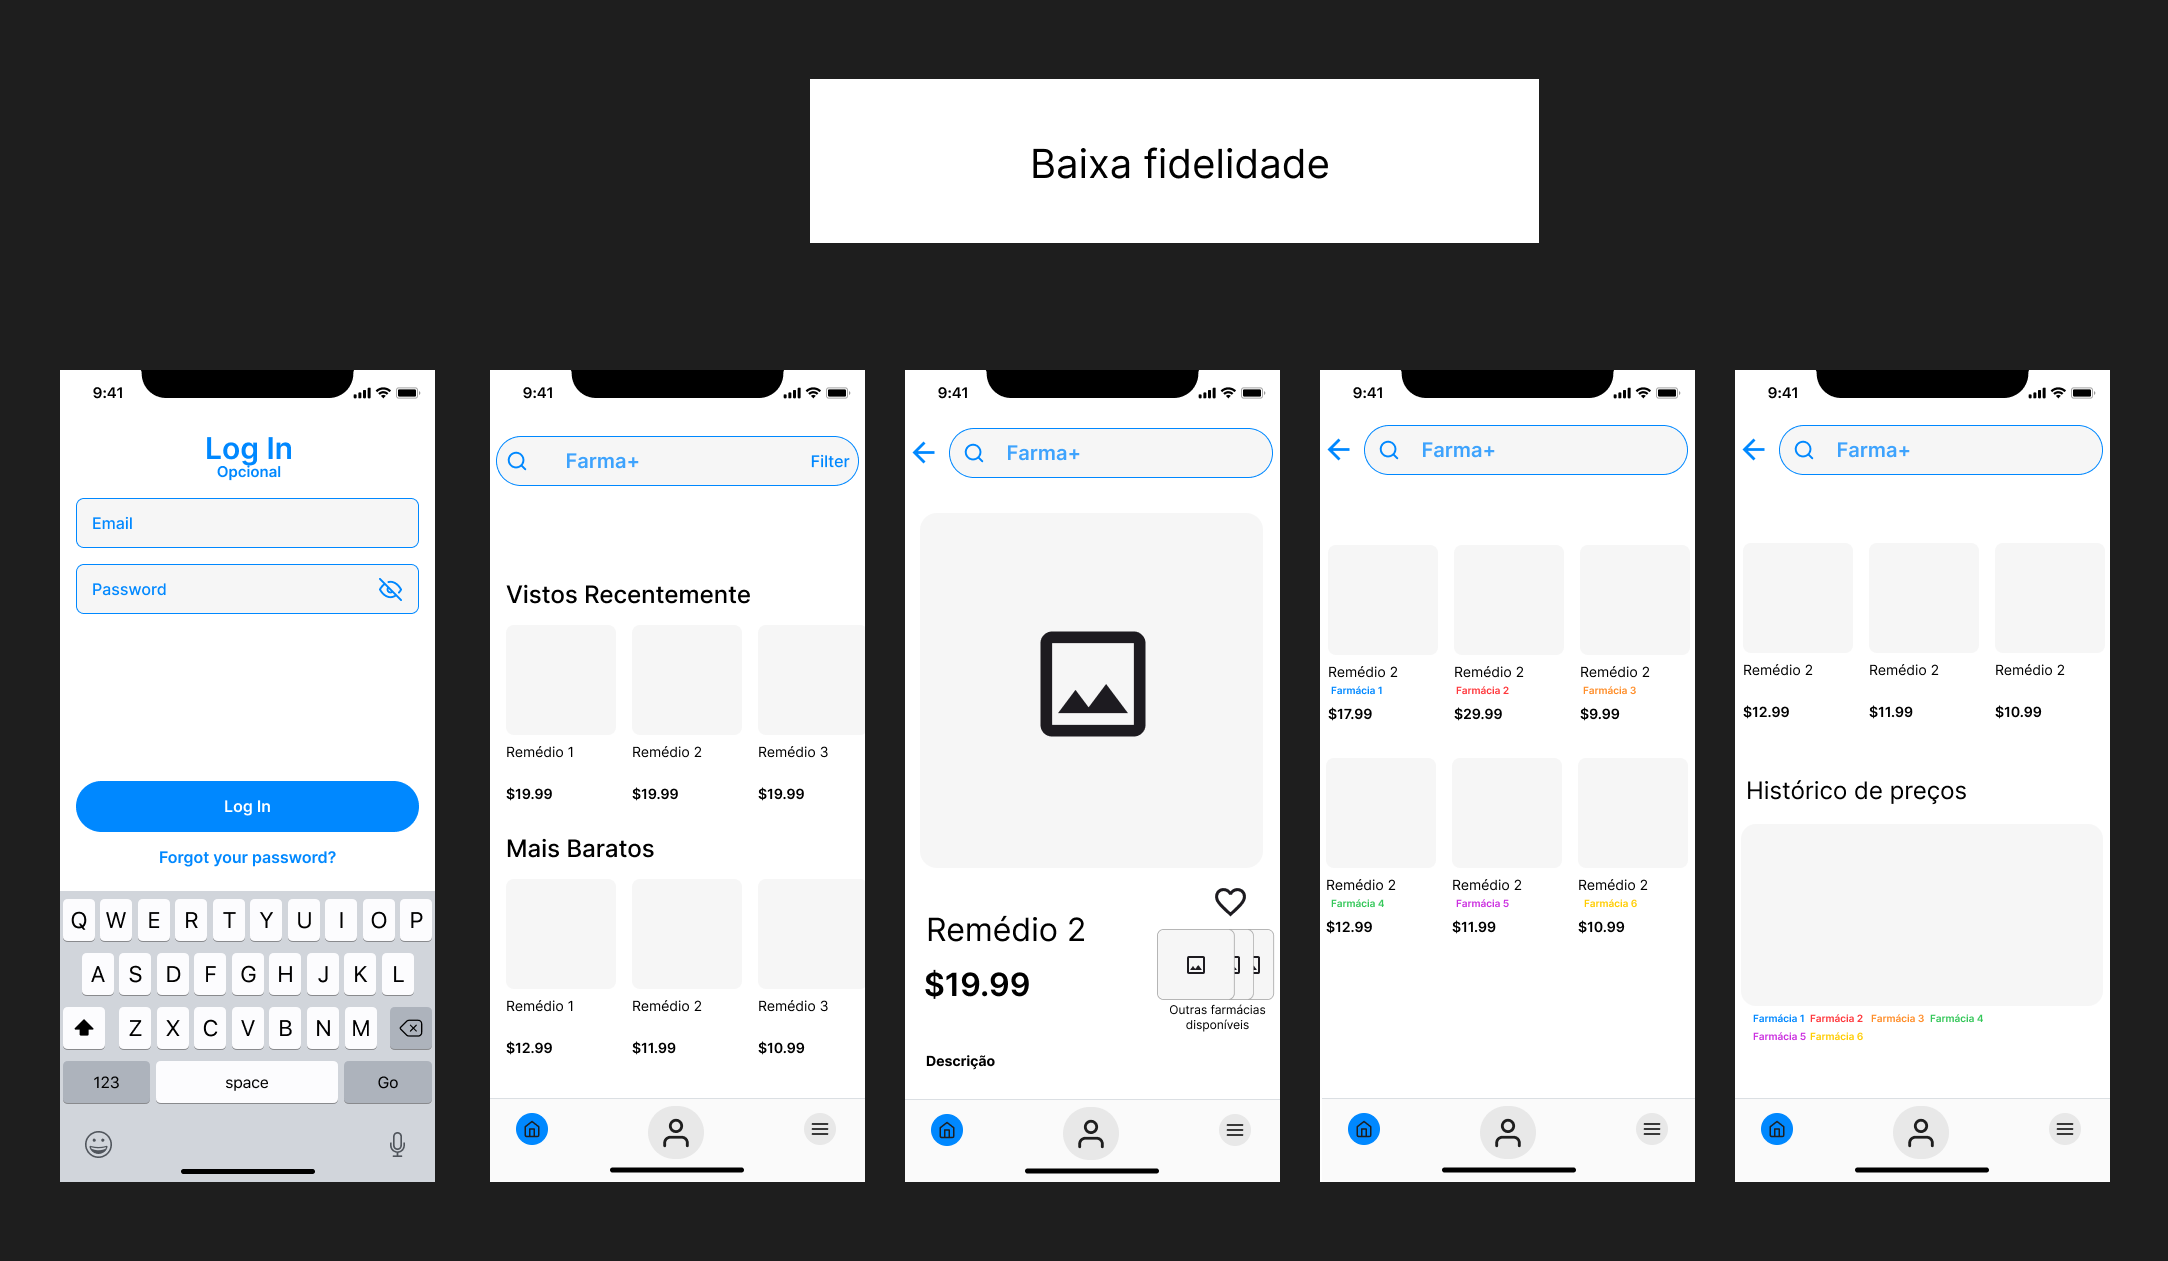
\includegraphics[width=0.45\textwidth,trim=57bp 72bp 1730bp 323bp,clip]{figures/prototipo-telas.png}\hfill
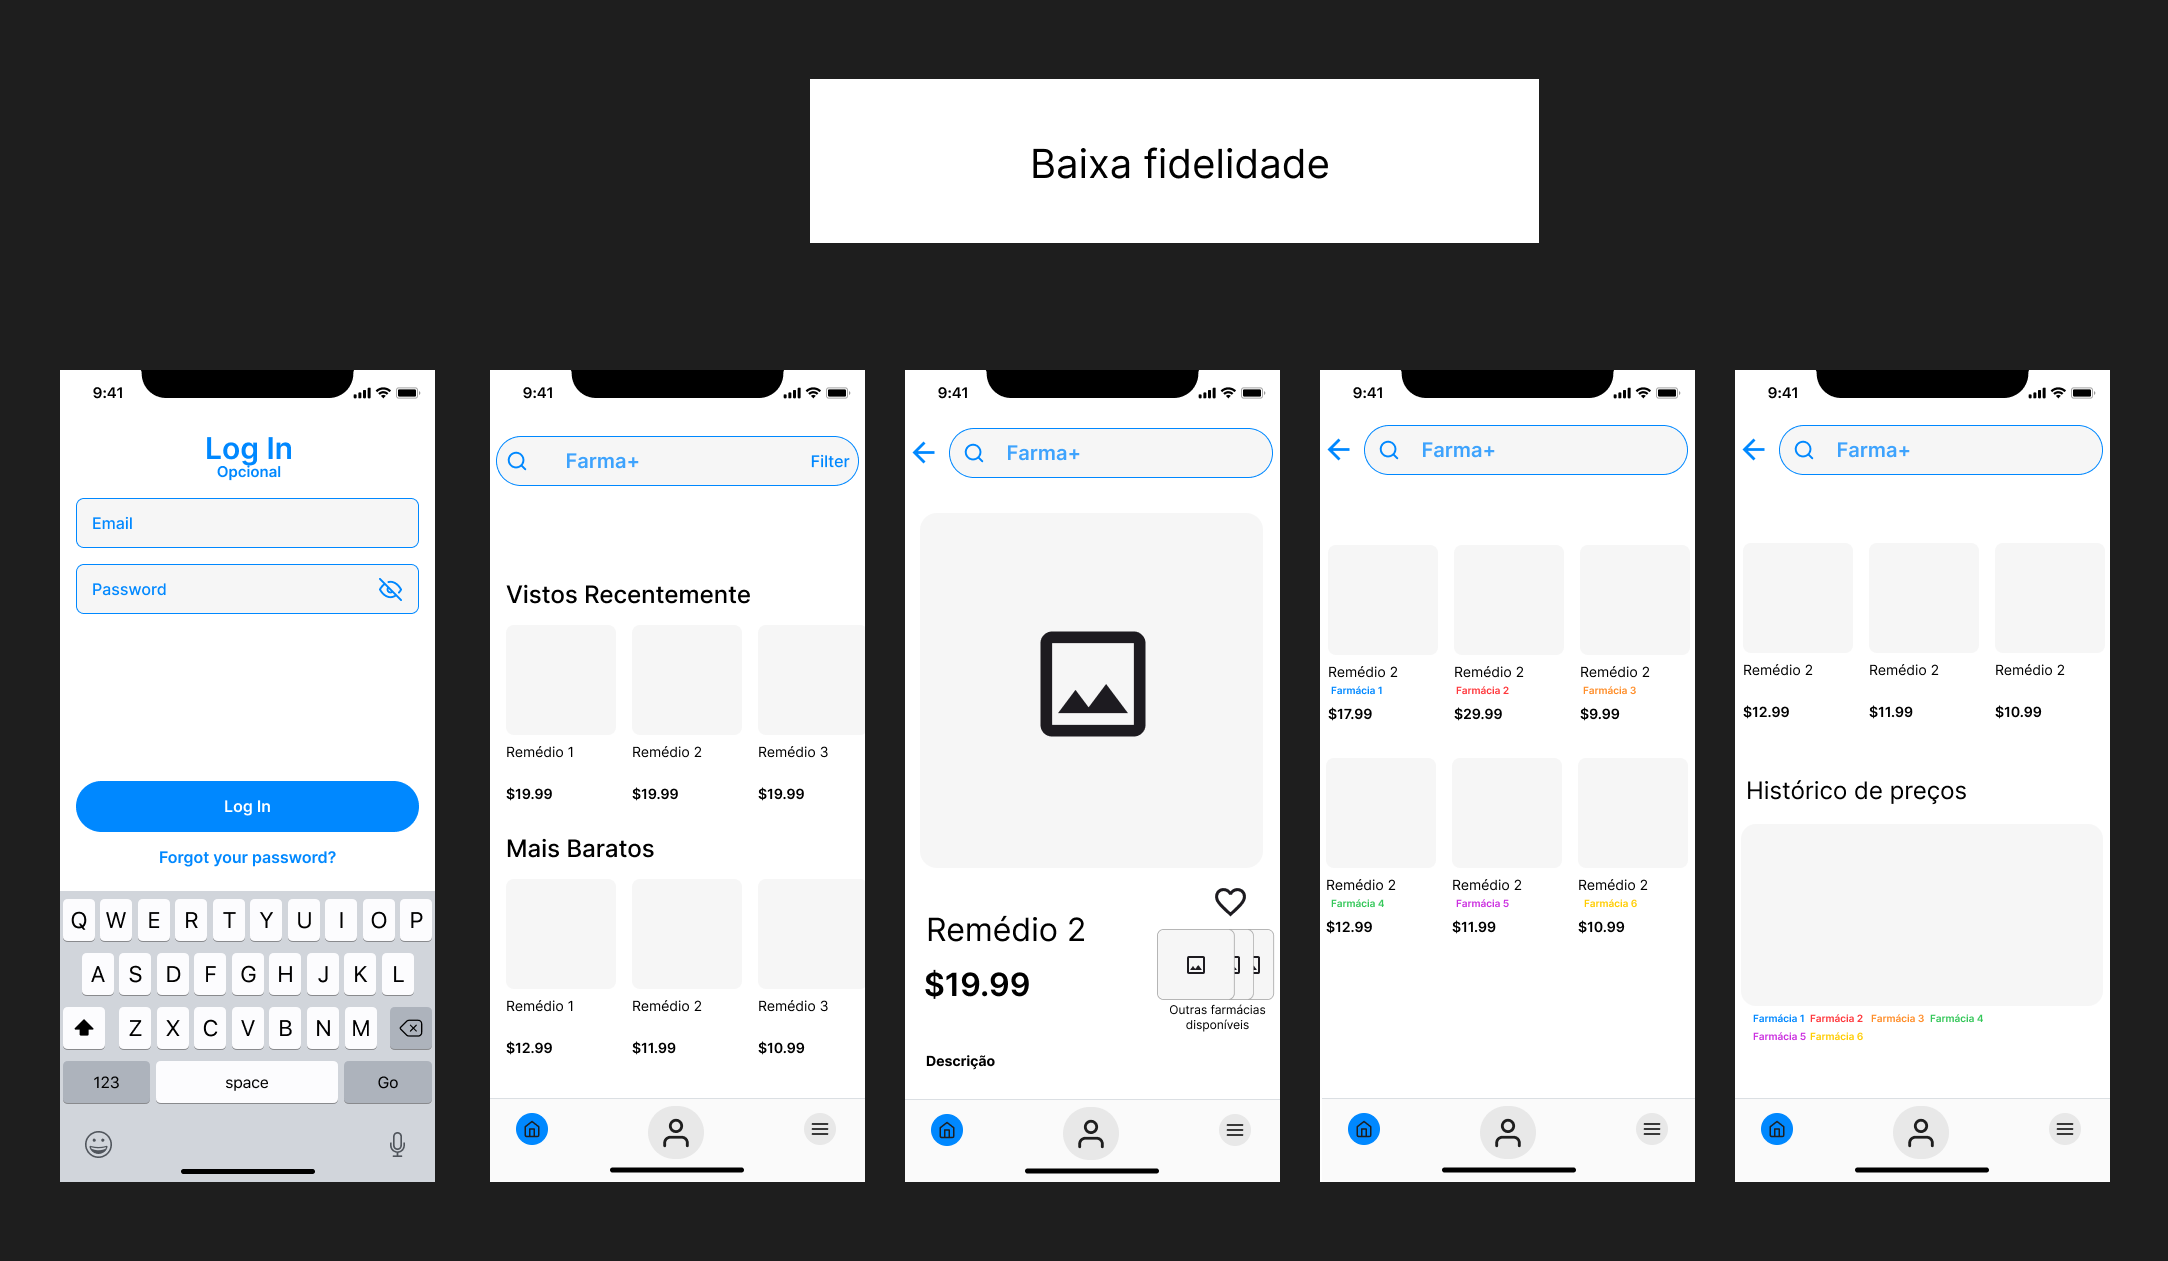
\includegraphics[width=0.45\textwidth,trim=487bp 72bp 1300bp 323bp,clip]{figures/prototipo-telas.png}
\fonte{Recortes do protótipo preservado no repositório.}
\end{figure}
\begin{figure}[p]
\centering\caption{Ampliação do protótipo: detalhe e pesquisa}\label{fig:prototipo_detalhe_busca}
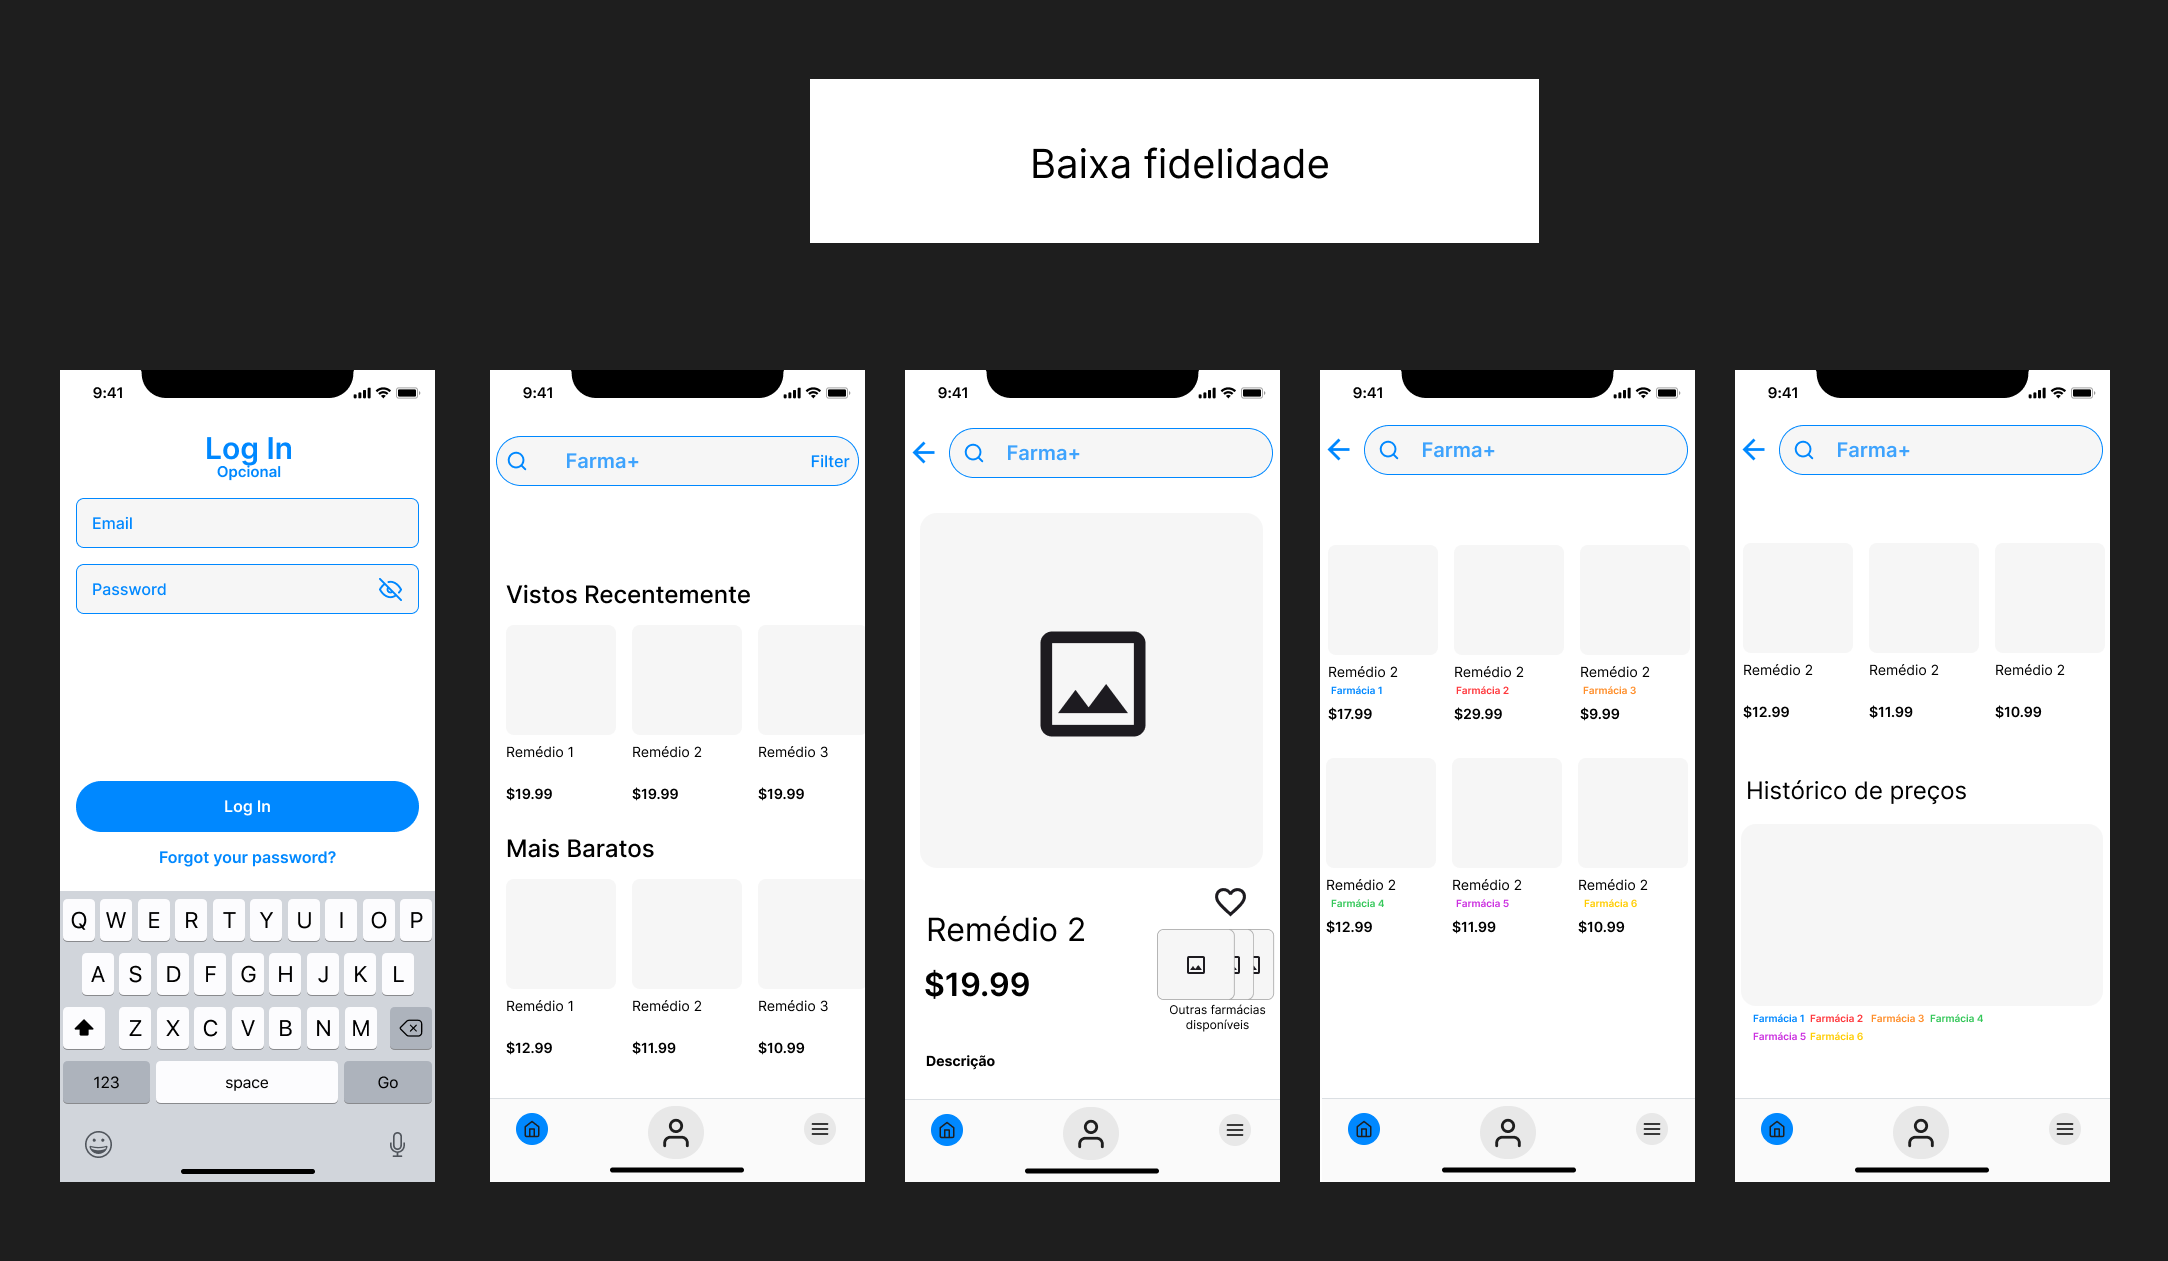
\includegraphics[width=0.45\textwidth,trim=902bp 72bp 885bp 323bp,clip]{figures/prototipo-telas.png}\hfill
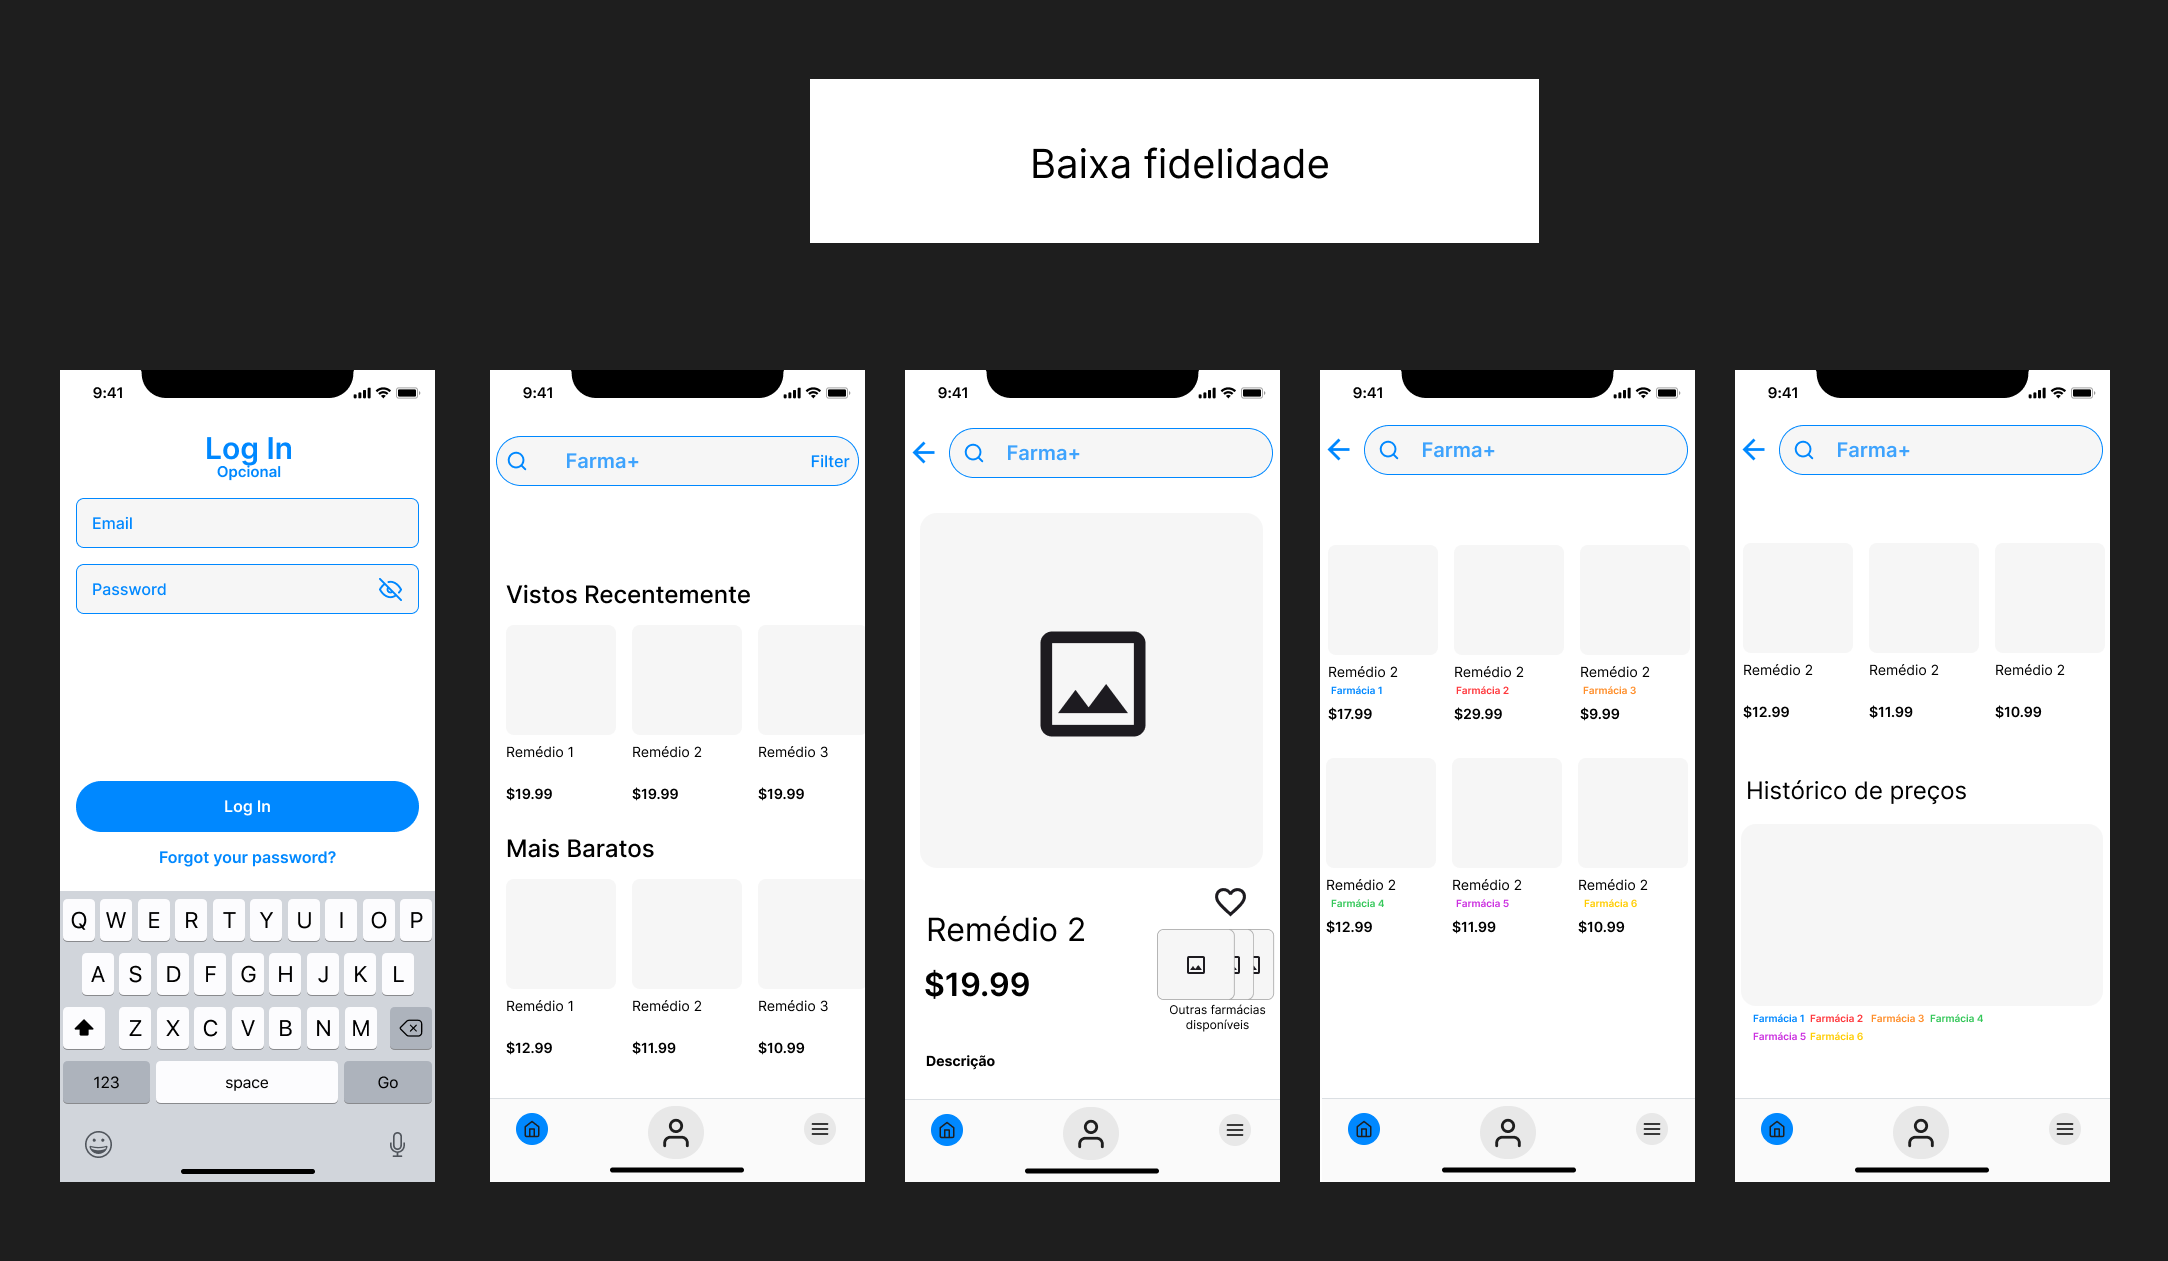
\includegraphics[width=0.45\textwidth,trim=1317bp 72bp 470bp 323bp,clip]{figures/prototipo-telas.png}
\fonte{Recortes do protótipo preservado no repositório.}
\end{figure}
\begin{figure}[p]
\centering\caption{Ampliação do protótipo: histórico de preços}\label{fig:prototipo_historico}
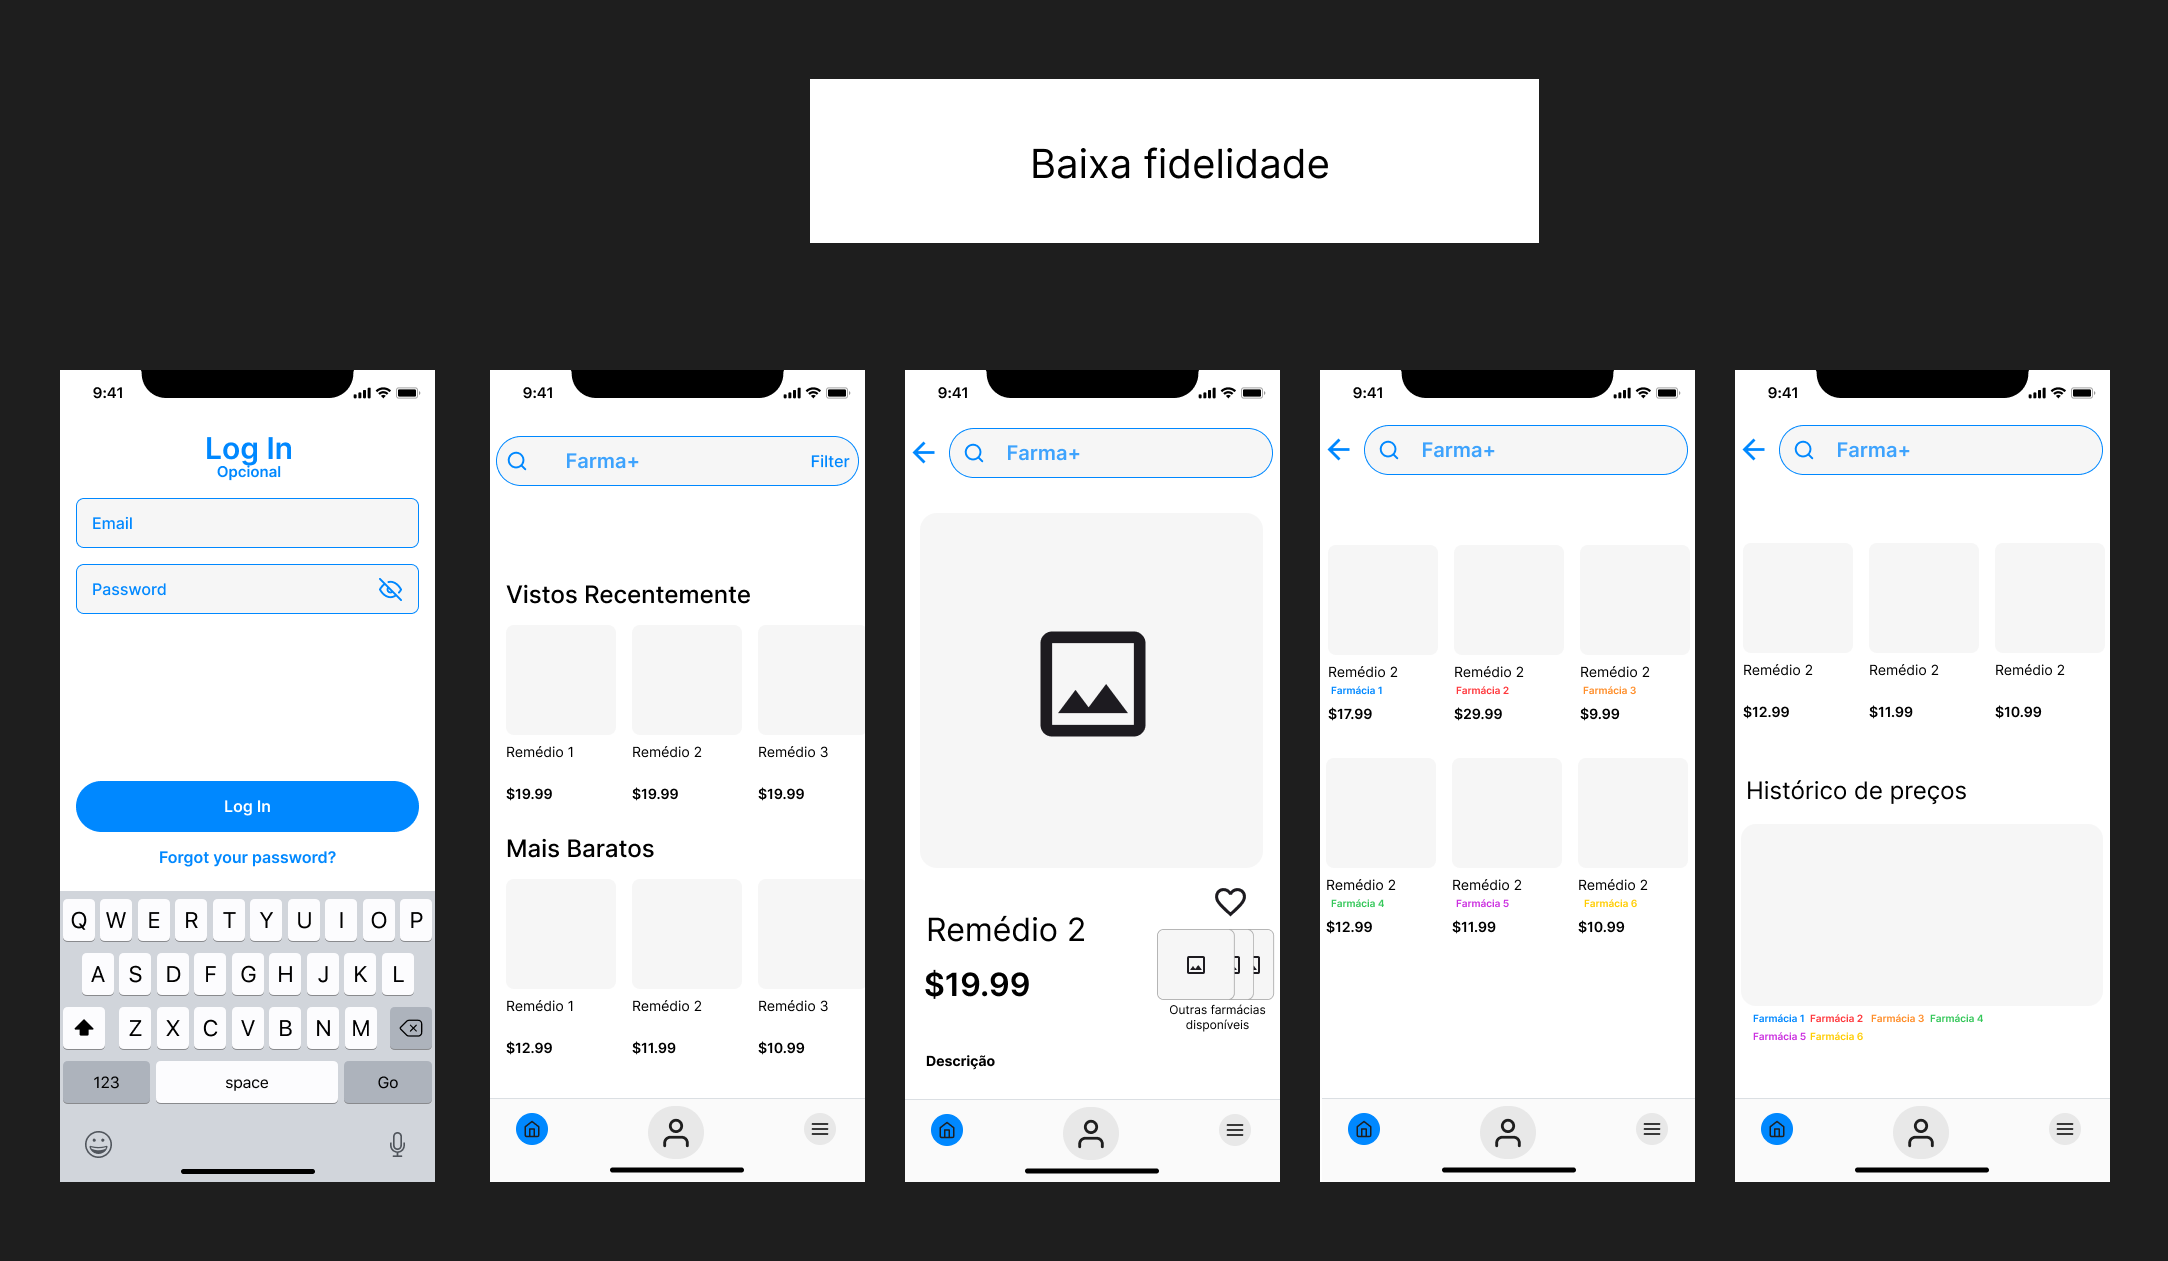
\includegraphics[width=0.45\textwidth,trim=1732bp 72bp 55bp 323bp,clip]{figures/prototipo-telas.png}
\fonte{Recorte do protótipo preservado no repositório.}
\end{figure}

A ordem real, da esquerda para a direita, é: login, início, detalhe do produto, resultados de busca e histórico. Login é opcional para consulta; favoritos e perfil requerem sessão ativa. O protótipo contém rótulos em inglês e valores ilustrativos; estes não são evidências de preços coletados.

\begin{itemize}
\item \textbf{Conta (UC03/RF03):} login solicita e-mail e senha e mostra opção de recuperação. A opção desenhada não comprova implementação de recuperação; as telas implementadas de login e cadastro estão em \file{frontend/src/app/}.
\item \textbf{Início e busca (UC04/RF04--RF05):} protótipo mostra pesquisa, itens e cartões. A implementação usa rotas de início e busca, filtros e \file{MedicineCard.tsx}. O detalhe apresenta ofertas; preço observado não garante disponibilidade física.
\item \textbf{Favoritos e histórico (UC06--UC07/RF07--RF08):} o coração no detalhe indica salvamento pretendido; a persistência atual é implementada pelos hooks de favoritos e pelas rotas autenticadas. A tela de histórico corresponde à consulta de séries, atualmente composta por \file{HistoryChart.tsx}.
\item \textbf{Distância (UC05/RF06):} permanece uma jornada prevista; não há fundamento para descrever quilometragem exata na imagem ou no fluxo implementado.
\end{itemize}

Não há ensaio de contraste, tamanho de alvos de toque ou navegação assistiva que sustente conformidade WCAG. Hierarquia visual e ícones são decisões de projeto; acessibilidade efetiva requer avaliação específica.

\FloatBarrier
\section{Plano de Testes} %

Este tópico apresenta o plano de testes da plataforma Preço Bão, mantendo alinhamento com a especificação de requisitos, modelagem, arquitetura e protótipo de interface documentados no projeto. O objetivo é planejar a verificação e validação das funcionalidades principais do sistema, incluindo pesquisa de medicamentos, comparação de preços, geolocalização, autenticação, favoritos, monitoramento de preços e rotina automatizada de coleta de dados por \textit{web scraping}.

\subsection{Introdução} %

\begin{itemize}
    \item \textbf{Nome do sistema:} Plataforma Preço Bão.
    \item \textbf{Objetivo do software:} Permitir que consumidores pesquisem, comparem e monitorem preços de medicamentos e produtos de farmácia por meio de aplicativo móvel e versão web.
    \item \textbf{Problema que o sistema busca resolver:} A dificuldade do consumidor em comparar preços de medicamentos em diferentes farmácias, considerando volatilidade dos valores, disponibilidade estimada em estoque e distância até os estabelecimentos.
    \item \textbf{Público-alvo:} Consumidores finais que compram medicamentos de uso contínuo, produtos de farmácia, higiene e dermocosméticos, especialmente usuários que desejam economizar tempo e dinheiro.
    \item \textbf{Integrantes do grupo:} Aurora Drumond Costa Magalhães, Ana Clara de Souza e Kayke Wellington Ribeiro Santos.
\end{itemize}

\subsection{Escopo dos Testes} %

O escopo dos testes contempla as funcionalidades centrais necessárias para validar o funcionamento do sistema sob a perspectiva do usuário final, do banco de dados e dos serviços de retaguarda.

\textbf{Funcionalidades que serão testadas:}
\begin{itemize}
    \item Cadastro, \textit{login}, autenticação e recuperação de senha de usuários.
    \item Pesquisa de medicamentos e produtos de farmácia.
    \item Exibição dos resultados em cartões padronizados, contendo laboratório, preço, farmácia, disponibilidade estimada e origem da oferta.
    \item Ordenação neutra dos resultados por menor preço ou menor distância.
    \item Cálculo de distância geográfica mediante autorização de localização.
    \item Favoritar medicamentos e produtos para acompanhamento posterior.
    \item Exibição de histórico ou gráfico de variação de preços.
    \item Rotina automatizada de \textit{web scraping}, tratamento de falhas e persistência dos dados coletados.
    \item Integração entre \textit{frontend} React Native, \textit{backend} FastAPI e banco PostgreSQL.
\end{itemize}

\textbf{Funcionalidades fora do escopo:}
\begin{itemize}
    \item Compra, pagamento ou reserva de medicamentos dentro da plataforma.
    \item Confirmação oficial de estoque em tempo real diretamente no sistema da farmácia.
    \item Entrega em domicílio ou integração com sistemas logísticos.
    \item Validação regulatória completa de prescrição médica ou controle de receita.
\end{itemize}

\textbf{Limitações identificadas:}
\begin{itemize}
    \item A disponibilidade em estoque é uma estimativa e deve ser confirmada no local pelo usuário.
    \item A precisão dos dados depende da qualidade das páginas públicas das farmácias e da rotina de extração.
    \item A geolocalização depende da permissão do usuário e da precisão do dispositivo.
    \item Testes de carga em ambiente acadêmico podem não representar a escala real de produção.
\end{itemize}

\subsection{Requisitos a Serem Testados} %

Os requisitos selecionados foram extraídos da especificação do projeto e representam os comportamentos funcionais e critérios de qualidade mais relevantes para a validação da plataforma.

\begingroup\footnotesize\def\LTcaptype{quadro}
\begin{xltabular}{\textwidth}{|c|Y|}
\caption{Requisitos funcionais selecionados para teste}\label{qua:testes_rf}\\
        \hline
        \textbf{ID} & \textbf{Requisito a ser testado} \\
        \hline\endfirsthead
\multicolumn{2}{l}{Quadro \thequadro\ -- continuação}\\
        \hline
        \textbf{ID} & \textbf{Requisito a ser testado} \\
        \hline\endhead
\multicolumn{2}{r}{Continua na próxima página.}\\\endfoot
\multicolumn{2}{l}{Fonte: Elaborado pelos autores (2026).}\\\endlastfoot

        RF01 & \textbf{Extração Resiliente de Dados:} validar se a rotina de \textit{web scraping} coleta dados de farmácias, registra falhas em \textit{log} e continua a varredura nas demais fontes. \\
        \hline
        RF02 & \textbf{Processamento e Catálogo:} verificar persistência, enriquecimento CMED/ANVISA e aviso de estoque estimado, incluindo ausência de correspondência. \\
        \hline
        RF03 & \textbf{Gestão de Usuários:} verificar cadastro, autenticação, \textit{login} e recuperação de senha do usuário. \\
        \hline
        RF04 & \textbf{Pesquisa e Neutralidade Algorítmica:} validar busca por medicamentos e ordenação por menor preço ou menor distância. \\
        \hline
        RF05 & \textbf{Exibição em Cartões:} verificar se os resultados são exibidos com informações de laboratório, preço e melhores ofertas. \\
        \hline
        RF06 & \textbf{Cálculo de Distância Geográfica:} verificar cálculo de distância até as farmácias após permissão de localização. \\
        \hline
        RF07 & \textbf{Salvamento de Produtos:} validar a opção de favoritar medicamentos de uso contínuo na conta do usuário. \\
        \hline
        RF08 & \textbf{Monitoramento de Preços:} verificar o histórico ou gráfico de flutuação de preços dos itens salvos. \\
        \hline
    \end{xltabular}
\endgroup

\begingroup\footnotesize\def\LTcaptype{quadro}
\begin{xltabular}{\textwidth}{|c|Y|}
\caption{Requisitos não funcionais selecionados para teste}\label{qua:testes_rnf}\\
        \hline
        \textbf{ID} & \textbf{Requisito a ser testado} \\
        \hline\endfirsthead
\multicolumn{2}{l}{Quadro \thequadro\ -- continuação}\\
        \hline
        \textbf{ID} & \textbf{Requisito a ser testado} \\
        \hline\endhead
\multicolumn{2}{r}{Continua na próxima página.}\\\endfoot
\multicolumn{2}{l}{Fonte: Elaborado pelos autores (2026).}\\\endlastfoot

        RNF01 & \textbf{Performance da API:} validar resposta de requisições de pesquisa em até 500 milissegundos no percentil 95. \\
        \hline
        RNF02 & \textbf{Arquitetura do Frontend:} verificar execução do aplicativo React Native/Expo com TypeScript para Android e iOS. \\
        \hline
        RNF04 & \textbf{Segurança e Criptografia:} validar armazenamento de senhas com \textit{hash} forte e comunicação protegida por HTTPS/TLS. \\
        \hline
        RNF05 & \textbf{Privacidade (LGPD):} verificar se coordenadas geográficas são processadas em memória e descartadas após uso. \\
        \hline
        RNF08 & \textbf{Orquestração Local:} validar provisionamento do ambiente com \file{docker-compose.yml}. \\
        \hline
        RNF10 & \textbf{CI/CD e Qualidade:} verificar bloqueio de \textit{Pull Requests} que falhem em testes ou análise estática. \\
        \hline
    \end{xltabular}
\endgroup

\subsection{Estratégia de Testes} %

A estratégia de testes combina validação funcional, integração, persistência, segurança, interface e desempenho, cobrindo tanto o fluxo do usuário quanto os componentes internos da arquitetura.

\begingroup\footnotesize\def\LTcaptype{quadro}
\begin{xltabular}{\textwidth}{|l|Y|Y|Y|}
\caption{Estratégias de teste propostas}\label{qua:estrategias_teste}\\
        \hline
        \textbf{Tipo de Teste} & \textbf{Objetivo} & \textbf{Técnica Utilizada} & \textbf{Resultado Esperado} \\
        \hline\endfirsthead
\multicolumn{4}{l}{Quadro \thequadro\ -- continuação}\\
        \hline
        \textbf{Tipo de Teste} & \textbf{Objetivo} & \textbf{Técnica Utilizada} & \textbf{Resultado Esperado} \\
        \hline\endhead
\multicolumn{4}{r}{Continua na próxima página.}\\\endfoot
\multicolumn{4}{l}{Fonte: Elaborado pelos autores (2026).}\\\endlastfoot

        Teste Funcional & Verificar se as funcionalidades do sistema executam corretamente conforme os requisitos. & Executar fluxos com dados válidos e inválidos em cadastro, \textit{login}, pesquisa, favoritos e histórico. & O sistema deve responder corretamente às ações do usuário e exibir mensagens adequadas. \\
        \hline
        Teste de Interface & Avaliar usabilidade, organização visual e navegação entre as telas. & Navegar pelo aplicativo validando botões, campos, cartões, barra inferior, contraste e rótulos. & As telas devem permitir concluir as jornadas avaliadas, com rótulos e ações legíveis, registrando dificuldades observadas. \\
        \hline
        Teste de Banco de Dados & Verificar persistência, consulta e integridade das informações. & Inserir, consultar e validar registros em Usuario, CatalogoBase, Farmacia, OfertaFarmacia, associações de favoritos e HistoricoPreco. & Os dados devem ser armazenados e recuperados sem inconsistências. \\
        \hline
        Teste de Segurança & Garantir proteção de credenciais e acesso restrito a recursos autenticados. & Testar \textit{login} inválido, acesso a favoritos sem autenticação, \textit{hash} de senha e descarte de localização. & Usuários não autorizados não devem acessar recursos restritos, e dados sensíveis não devem ser expostos. \\
        \hline
        Teste de Integração & Verificar comunicação entre \textit{frontend}, API, banco e rotina de \textit{scraping}. & Executar fluxo completo: coleta de dados, gravação no PostgreSQL, consulta via FastAPI e exibição no app. & Os módulos devem trocar informações corretamente e tratar falhas sem interromper o sistema. \\
        \hline
        Teste de Desempenho & Avaliar comportamento da API em pesquisas simultâneas. & Simular múltiplas requisições e medir tempo de resposta das buscas principais. & A API deve manter tempo de resposta compatível com RNF01. \\
        \hline
    \end{xltabular}
\endgroup

\subsection{Casos de Teste} %

Os casos de teste foram definidos para cobrir os fluxos principais da plataforma. Todos permanecem \textbf{Pendentes}: os resultados descritos são esperados, não observados. CT13 foi detalhado para incluir RF02 e CT14 para explicitar o critério de RNF01; esses detalhamentos pertencem à consolidação documental, sem execução histórica atribuída à equipe.

A rastreabilidade funcional é: RF01--CT12; RF02--CT13; RF03--CT01/CT02/CT03 (recuperação de senha ainda sem caso específico); RF04--CT04/CT05/CT06/CT07; RF05--CT04; RF06--CT07/CT08; RF07--CT09/CT10; RF08--CT11. A cobertura de RNF01 está em CT14. Hash, HTTPS, descarte de localização, orquestração e bloqueio de PRs aparecem nas estratégias, mas carecem de procedimentos e registros específicos. Assim, a seleção de requisitos não equivale a cobertura integral validada.

\begingroup\footnotesize\def\LTcaptype{quadro}
\begin{xltabular}{\textwidth}{|c|Y|Y|Y|}
\caption{Casos de teste da plataforma Preço Bão - Prioridade Alta}\label{qua:casos_teste_alta}\\
        \hline
        \textbf{ID} & \textbf{Caso de Teste} & \textbf{Entrada de Dados} & \textbf{Resultado Esperado} \\
        \hline\endfirsthead
\multicolumn{4}{l}{Quadro \thequadro\ -- continuação}\\
        \hline
        \textbf{ID} & \textbf{Caso de Teste} & \textbf{Entrada de Dados} & \textbf{Resultado Esperado} \\
        \hline\endhead
\multicolumn{4}{r}{Continua na próxima página.}\\\endfoot
\multicolumn{4}{l}{Fonte: Elaborado pelos autores (2026).}\\\endlastfoot

        CT01 & Cadastro de usuário com dados válidos & Nome, e-mail válido e senha válida & Usuário cadastrado com sucesso e perfil criado. \\
        \hline
        CT02 & Login com credenciais válidas & E-mail e senha corretos & Acesso permitido à conta do usuário. \\
        \hline
        CT03 & Login com senha inválida & E-mail válido e senha incorreta & Sistema deve negar acesso e exibir mensagem de credenciais inválidas. \\
        \hline
        CT04 & Pesquisa de medicamento existente & Nome de medicamento presente no catálogo & Sistema deve listar ofertas disponíveis em cartões padronizados. \\
        \hline
        CT06 & Ordenação por menor preço & Busca com múltiplas ofertas & Resultados devem ser ordenados pelo menor preço, sem favorecimento de farmácia. \\
        \hline
        CT07 & Ordenação por menor distância & Busca com permissão de localização ativa & Resultados devem ser ordenados pela menor distância calculada até as farmácias. \\
        \hline
        CT09 & Favoritar medicamento autenticado & Usuário logado seleciona favorito & Produto deve ser associado ao usuário e aparecer na tela de favoritos. \\
        \hline
        CT10 & Favoritar medicamento sem login & Usuário não autenticado tenta favoritar & Sistema deve solicitar login antes de salvar o produto. \\
        \hline
        CT12 & Scraping com falha parcial & Uma fonte indisponível durante a coleta & Erro deve ser registrado em log e a varredura deve continuar nas demais farmácias. \\
        \hline
        CT13 & Persistência de oferta coletada & Produto, farmácia, preço e disponibilidade coletados & Dados devem ser gravados em OfertaFarmacia e vinculados ao catálogo e à farmácia; conferir enriquecimento CMED/ANVISA, ausência de correspondência e aviso de estoque estimado (RF02). \\
        \hline
    \end{xltabular}
\endgroup

\begingroup\footnotesize\def\LTcaptype{quadro}
\begin{xltabular}{\textwidth}{|c|Y|Y|Y|}
\caption{Casos de teste da plataforma Preço Bão - Prioridade Média}\label{qua:casos_teste_media}\\
        \hline
        \textbf{ID} & \textbf{Caso de Teste} & \textbf{Entrada de Dados} & \textbf{Resultado Esperado} \\
        \hline\endfirsthead
\multicolumn{4}{l}{Quadro \thequadro\ -- continuação}\\
        \hline
        \textbf{ID} & \textbf{Caso de Teste} & \textbf{Entrada de Dados} & \textbf{Resultado Esperado} \\
        \hline\endhead
\multicolumn{4}{r}{Continua na próxima página.}\\\endfoot
\multicolumn{4}{l}{Fonte: Elaborado pelos autores (2026).}\\\endlastfoot

        CT05 & Pesquisa sem resultado & Nome inexistente ou inválido & Sistema deve informar que nenhum produto foi encontrado. \\
        \hline
        CT08 & Negar permissão de localização & Usuário recusa acesso à localização & Sistema deve manter pesquisa por preço e informar indisponibilidade da ordenação por distância. \\
        \hline
        CT11 & Exibir histórico de preços & Produto salvo com registros em HistoricoPreco & Sistema deve apresentar gráfico ou lista de variação de preços das últimas semanas. \\
        \hline
    \end{xltabular}
\endgroup

\begingroup\footnotesize\def\LTcaptype{quadro}
\begin{xltabular}{\textwidth}{|c|Y|Y|Y|}
\caption{Casos de teste da plataforma Preço Bão - Prioridade Baixa}\label{qua:casos_teste_baixa}\\
        \hline
        \textbf{ID} & \textbf{Caso de Teste} & \textbf{Entrada de Dados} & \textbf{Resultado Esperado} \\
        \hline\endfirsthead
\multicolumn{4}{l}{Quadro \thequadro\ -- continuação}\\
        \hline
        \textbf{ID} & \textbf{Caso de Teste} & \textbf{Entrada de Dados} & \textbf{Resultado Esperado} \\
        \hline\endhead
\multicolumn{4}{r}{Continua na próxima página.}\\\endfoot
\multicolumn{4}{l}{Fonte: Elaborado pelos autores (2026).}\\\endlastfoot

        CT14 & Teste de desempenho da busca & Múltiplas requisições simultâneas de pesquisa & O percentil 95 dos tempos de resposta deve ser menor ou igual a 500 ms (RNF01); registrar carga, ambiente, duração, amostra e método de cálculo. \\
        \hline
    \end{xltabular}
\endgroup

\subsection{Infraestrutura e Recursos de Teste} %

\begin{itemize}
    \item \textbf{Sistema operacional:} Windows 10/11 ou Linux para execução dos serviços de desenvolvimento e testes.
    \item \textbf{Banco de dados:} PostgreSQL, conforme especificação de persistência do projeto.
    \item \textbf{Backend:} Python com FastAPI, SQLAlchemy ORM, Pydantic e execução assíncrona.
    \item \textbf{Frontend:} React Native com Expo e TypeScript.
    \item \textbf{Navegador:} Google Chrome, Microsoft Edge ou navegador compatível para validação da versão web e consumo da API.
    \item \textbf{Ferramentas:} Visual Studio Code, Docker, docker-compose, Git/GitHub, GitHub Actions, ESLint, Ruff e ferramentas de teste da API.
    \item \textbf{Equipamentos:} Computador de desenvolvimento e smartphone ou emulador Android/iOS para validação do aplicativo móvel.
\end{itemize}

\subsection{Equipe e Responsabilidades} %

O quadro preserva a distribuição de responsabilidades registrada no plano. As funções são atribuições planejadas; não comprovam execução, participação ou resultados individuais.

\begingroup\footnotesize\def\LTcaptype{quadro}
\begin{xltabular}{\textwidth}{|l|Y|}
\caption{Equipe e responsabilidades}\label{qua:equipe_responsabilidades}\\
        \hline
        \textbf{Integrante} & \textbf{Função} \\
        \hline\endfirsthead
\multicolumn{2}{l}{Quadro \thequadro\ -- continuação}\\
        \hline
        \textbf{Integrante} & \textbf{Função} \\
        \hline\endhead
\multicolumn{2}{r}{Continua na próxima página.}\\\endfoot
\multicolumn{2}{l}{Fonte: Elaborado pelos autores (2026).}\\\endlastfoot

        Aurora Drumond Costa Magalhães & Elaboração dos casos de teste e validação dos requisitos funcionais. \\
        \hline
        Ana Clara de Souza & Execução dos testes de interface, autenticação, favoritos e registro das falhas encontradas. \\
        \hline
        Kayke Wellington Ribeiro Santos & Execução dos testes de \textit{backend}, banco de dados, \textit{scraping}, desempenho e integração. \\
        \hline
        Grupo & Revisão final do plano de testes, consolidação dos resultados e validação do documento. \\
        \hline
    \end{xltabular}
\endgroup

\subsection{Cronograma de Testes} %

O cronograma a seguir preserva as datas e atribuições do plano. A ordem das linhas não é estritamente cronológica: as etapas de 13 e 14 de junho antecedem a execução funcional e de interface de 16 de junho. Sem registros de execução, não se presume que as datas estejam erradas nem que o registro de falhas de 14 de junho abranja a etapa posterior.

\begingroup\footnotesize\def\LTcaptype{quadro}
\begin{xltabular}{\textwidth}{|Y|l|c|}
\caption{Cronograma simplificado de testes}\label{qua:cronograma_testes}\\
        \hline
        \textbf{Atividade} & \textbf{Responsável} & \textbf{Prazo} \\
        \hline\endfirsthead
\multicolumn{3}{l}{Quadro \thequadro\ -- continuação}\\
        \hline
        \textbf{Atividade} & \textbf{Responsável} & \textbf{Prazo} \\
        \hline\endhead
\multicolumn{3}{r}{Continua na próxima página.}\\\endfoot
\multicolumn{3}{l}{Fonte: Elaborado pelos autores (2026).}\\\endlastfoot

        Planejamento dos testes & Grupo & 03/06/2026 \\
        \hline
        Elaboração dos casos de teste & Aurora Drumond Costa Magalhães & 08/06/2026 \\
        \hline
        Preparação do ambiente de teste & Kayke Wellington Ribeiro Santos & 12/06/2026 \\
        \hline
        Execução dos testes funcionais e de interface & Ana Clara de Souza & 16/06/2026 \\
        \hline
        Execução dos testes de banco, integração, segurança e desempenho & Kayke Wellington Ribeiro Santos & 13/06/2026 \\
        \hline
        Registro de falhas e análise dos riscos & Grupo & 14/06/2026 \\
        \hline
        Correção, validação e revisão final & Grupo & 17/06/2026 \\
        \hline
    \end{xltabular}
\endgroup

\subsection{Registro de Defeitos e Riscos} %

O registro de defeitos e riscos é prospectivo e não relata falhas reproduzidas. Ele antecipa problemas que podem ocorrer durante a execução dos testes e durante a evolução do projeto.

\begingroup\footnotesize\def\LTcaptype{quadro}
\begin{xltabular}{\textwidth}{|c|Y|Y|Y|}
\caption{Hipóteses de defeitos para investigação}\label{qua:defeitos_identificados}\\
        \hline
        \textbf{ID} & \textbf{Hipótese de falha} & \textbf{Possível Causa} & \textbf{Solução Proposta} \\
        \hline\endfirsthead
\multicolumn{4}{l}{Quadro \thequadro\ -- continuação}\\
        \hline
        \textbf{ID} & \textbf{Hipótese de falha} & \textbf{Possível Causa} & \textbf{Solução Proposta} \\
        \hline\endhead
\multicolumn{4}{r}{Continua na próxima página.}\\\endfoot
\multicolumn{4}{l}{Fonte: Elaborado pelos autores (2026).}\\\endlastfoot

        RFAL01 & Login não permite acesso mesmo com credenciais corretas. & Erro na validação da senha, \textit{hash} incorreto ou falha de comunicação com o banco. & Revisar autenticação, geração de \textit{hash} e consulta do usuário no \textit{backend}. \\
        \hline
        RFAL02 & Pesquisa retorna produtos duplicados ou sem preço. & Falha no tratamento dos dados coletados pelo \textit{scraping} ou inconsistência em OfertaFarmacia. & Revisar normalização do catálogo, chaves de relacionamento e filtros da consulta. \\
        \hline
        RFAL03 & Distância geográfica exibida incorretamente. & Erro no cálculo de latitude/longitude, permissão negada ou coordenadas inválidas. & Validar fórmula de cálculo, tratar ausência de localização e testar valores conhecidos. \\
        \hline
        RFAL04 & Histórico de preços não aparece para produto favoritado. & Ausência de registros em HistoricoPreco ou erro de vínculo com usuário/produto. & Revisar rotina de gravação histórica e relacionamento entre as associações de favoritos e CatalogoBase. \\
        \hline
    \end{xltabular}
\endgroup

\begingroup\footnotesize\def\LTcaptype{quadro}
\begin{xltabular}{\textwidth}{|c|Y|Y|Y|}
\caption{Riscos relacionados ao projeto e aos testes}\label{qua:riscos_projeto}\\
        \hline
        \textbf{ID} & \textbf{Risco identificado} & \textbf{Impacto} & \textbf{Mitigação} \\
        \hline\endfirsthead
\multicolumn{4}{l}{Quadro \thequadro\ -- continuação}\\
        \hline
        \textbf{ID} & \textbf{Risco identificado} & \textbf{Impacto} & \textbf{Mitigação} \\
        \hline\endhead
\multicolumn{4}{r}{Continua na próxima página.}\\\endfoot
\multicolumn{4}{l}{Fonte: Elaborado pelos autores (2026).}\\\endlastfoot

        R01 & Mudança no layout ou na estrutura dos sites das farmácias. & Pode interromper ou reduzir a qualidade da extração de dados por \textit{scraping}. & Criar \textit{logs} detalhados, testes automatizados para os \textit{scrapers} e estratégia de adaptação por farmácia. \\
        \hline
        R02 & Ambiente de testes diferente do ambiente real de produção. & Resultados de desempenho e integração podem não representar a operação real. & Documentar limitações, executar testes em ambiente controlado e repetir cenários críticos em infraestrutura próxima da final. \\
        \hline
        R03 & Exposição indevida de dados pessoais ou localização. & Pode causar não conformidade com a LGPD e perda de confiança do usuário. & Validar descarte das coordenadas, revisar permissões e testar fluxos de privacidade. \\
        \hline
    \end{xltabular}
\endgroup